% !TEX program = xelatex
% !BIB program = bibtex
\documentclass[a4paper, 12pt, openany]{book}

% ===================== 1. 宏包加载 =====================
\usepackage[UTF8, heading=true]{ctex}
\usepackage{geometry}
\usepackage{fontspec}
\usepackage{titletoc}
\usepackage{titlesec}
\usepackage{fancyhdr}
\usepackage{graphicx}
\usepackage{booktabs} % 三线表
\usepackage{array}
\usepackage{amsmath, amssymb, amsfonts}
\usepackage{caption}
\usepackage{subcaption}
\usepackage{enumitem}
\usepackage{hyperref}
\usepackage{xcolor}
\usepackage{listings}
\usepackage[sort&compress]{gbt7714} % 国标参考文献支持
\usepackage{pdfpages}
\usepackage{makecell} % 表格换行
\usepackage{calc}
\usepackage{float}
\usepackage{algorithm}
\usepackage{algorithmic} % 提供 algorithmic 环境
\usepackage[table]{xcolor}
\usepackage{multirow}

% ===================== 2. 页面设置 (十九) =====================
% 上边距为25mm，下边距为20mm，左边距为30mm，右边距为30mm
\geometry{
	top=25mm,
	bottom=25mm,
	left=30mm,
	right=30mm,
	headheight=1.5cm,
	footskip=1.5cm
}

% ===================== 3. 字体与字号设置 (三) =====================
% 英文字体配置
\setmainfont{Times New Roman}
\setsansfont{Arial}
\setmonofont{Courier New}

% 字号命令（严格对应Word字号）
\newcommand{\yihao}{\fontsize{26pt}{31.2pt}\selectfont}
\newcommand{\erhao}{\fontsize{22pt}{26.4pt}\selectfont}      % 2号
\newcommand{\xiaoer}{\fontsize{18pt}{21.6pt}\selectfont}     % 小2号
\newcommand{\sanhao}{\fontsize{16pt}{19.2pt}\selectfont}     % 3号
\newcommand{\xiaosan}{\fontsize{15pt}{18pt}\selectfont}      % 小3号
\newcommand{\sihao}{\fontsize{14pt}{16.8pt}\selectfont}      % 4号
\newcommand{\xiaosi}{\fontsize{12pt}{14.4pt}\selectfont}     % 小4号 (正文默认)
\newcommand{\wuhao}{\fontsize{10.5pt}{12.6pt}\selectfont}    % 5号
\newcommand{\xiaowu}{\fontsize{9pt}{10.8pt}\selectfont}      % 小5号

% 行距设置：标题以外的文字行距为“固定值”23磅
\setlength{\baselineskip}{23pt} 

% ===================== 4. 章节标题格式 (三、六、九) =====================
\ctexset{
	chapter = {
		format = {\centering\heiti\xiaoer}, % 章标题 黑体小2号 居中
		name = {第,章},
		number = \arabic{chapter},
		aftername = \quad,
		beforeskip = -0.2\baselineskip, % 段前0.8行
		afterskip = 0.3\baselineskip,  % 段后0.5行
		pagestyle = fancy
	},
	section = {
		format = {\heiti\sihao},       % 一级标题 黑体4号
		aftername = \quad,
		beforeskip = 0.2\baselineskip, % 段前0.5行
		afterskip = 0.2\baselineskip   % 段后0.5行
	},
	subsection = {
		format = {\heiti\xiaosi},      % 二级标题 黑体小4号
		aftername = \quad,
		beforeskip = 0.2\baselineskip,
		afterskip = 0.2\baselineskip
	},
	subsubsection = {
		format = {\heiti\xiaosi},      % 三级标题 黑体小4号
		aftername = \quad,
		beforeskip = 0.2\baselineskip,
		afterskip = 0.2\baselineskip
	}
}

% ===================== 5. 目录格式 (八) =====================
% 目录标题：黑体小2号 (由ctexset chapter控制)
% 目录内容中章的标题：黑体4号
% 目录中其他内容：宋体小4号
% 页码：Times New Roman 5号

\titlecontents{chapter}[0em]
{\vspace{6pt}\heiti\sihao} % 章标题 黑体4号
{\thecontentslabel\quad}
{}
{\titlerule*[0.5pc]{$\cdot$}\rmfamily\wuhao\thecontentspage} % 页码 TNR 5号

\titlecontents{section}[2em]
{\songti\xiaosi}           % 节标题 宋体小4号
{\thecontentslabel\quad}
{}
{\titlerule*[0.5pc]{$\cdot$}\rmfamily\wuhao\thecontentspage}

\titlecontents{subsection}[4em]
{\songti\xiaosi}           % 条标题 宋体小4号
{\thecontentslabel\quad}
{}
{\titlerule*[0.5pc]{$\cdot$}\rmfamily\wuhao\thecontentspage}

% ===================== 6. 页眉页脚 (三) =====================
\pagestyle{fancy}
\fancyhf{}
% 论文页码 页脚居中、阿拉伯数字（Times new roman 5号）连续编码
\fancyfoot[C]{\rmfamily\wuhao\thepage} 
\renewcommand{\headrulewidth}{0.5pt}
% 按照示例，页眉通常为论文题目或“武汉大学...”，此处设为论文题目
\fancyhead[C]{\songti\xiaowu 武汉大学2026年自强杯大学生创业计划竞赛商业计划书}

\fancypagestyle{plain}{
	\fancyhf{}
	\fancyfoot[C]{\rmfamily\wuhao\thepage}
	\fancyhead[C]{\songti\xiaowu 武汉大学2026年自强杯大学生创业计划竞赛商业计划书}
	\renewcommand{\headrulewidth}{0.5pt}
}

% ===================== 7. 图表公式设置 (十二、十四、十五、十六) =====================
% 公式序号按章编排 (3.2)
\numberwithin{equation}{chapter}
\renewcommand{\theequation}{\thechapter.\arabic{equation}}

% 图表序号按章编排 图1.4 表2.4
\numberwithin{figure}{chapter}
\numberwithin{table}{chapter}
\renewcommand{\thefigure}{\thechapter.\arabic{figure}}
\renewcommand{\thetable}{\thechapter.\arabic{table}}

% 图表标题字体：黑体小4号，数字TNR粗体小4号
\DeclareCaptionFont{whucaption}{\heiti\xiaosi}
\captionsetup{
	font=whucaption,
	labelsep=quad,
	labelfont=bf, % 粗体
	textfont=normalfont
}
\captionsetup[figure]{name={图}}
\captionsetup[table]{name={表}}

% ===================== 8. 列表与引用设置 =====================
\setlist[itemize]{noitemsep, topsep=0pt, parsep=0pt}
\setlist[enumerate]{noitemsep, topsep=0pt, parsep=0pt}

% 引文标示：方括号上标，小4号 (gbt7714宏包已处理上标，此处微调字体)
\citestyle{super}

% 超链接颜色（打印时通常为黑色）
\hypersetup{
	colorlinks = true,
	linkcolor = black,
	citecolor = black,
	urlcolor = black,
	bookmarksnumbered = true,
	pdfstartview = FitH
}

% ===================== 9. 代码环境设置 =====================
\definecolor{codebg}{RGB}{248,248,248}
\definecolor{codeframe}{RGB}{220,220,220}
\definecolor{codecomment}{RGB}{0,128,0}
\definecolor{codekeyword}{RGB}{0,0,255}
\definecolor{codestring}{RGB}{163,21,21}

\lstset{
	basicstyle=\small\ttfamily,
	breaklines=true,
	frame=leftline,                    % 左侧线条
	framerule=3pt,                     % 线条粗细
	rulecolor=\color{codeframe},       % 线条颜色
	numbers=none,                      % 不显示行号
	tabsize=5,
	captionpos=b,
	backgroundcolor=\color{codebg},    % 背景色
	commentstyle=\color{codecomment}\itshape,    % 注释样式
	keywordstyle=\color{codekeyword}\bfseries,   % 关键字样式
	stringstyle=\color{codestring},              % 字符串样式
	xleftmargin=0pt,                   % 左边距（靠左对齐）
	xrightmargin=5pt,                  % 右边距
	aboveskip=10pt,                    % 上边距
	belowskip=10pt                     % 下边距
}

% ===================== 10. 自定义信息 =====================
\newcommand{\projectid}{}
\newcommand{\titlecn}{面向Aliro演进方向的后量子门禁认证方案} % 论文题目
\newcommand{\titleen}{Hardware-Accelerated Multi-Standard Post-Quantum Cryptography Library: Implementation and Optimization}
\newcommand{\college}{国家网络安全学院}
\newcommand{\major}{密码科学与技术}
\newcommand{\advisorone}{何德彪\quad 教授}
\newcommand{\advisortwo}{李小红\quad 副教授}
\newcommand{\advisorthree}{彭聪\quad 副教授}
\newcommand{\advisorfour}{冯琦\quad 副教授}
\newcommand{\advisorfive}{罗敏\quad 教授}
\newcommand{\reportdate}{二〇二六年三月}
\newcommand{\reportdateen}{March 2026}
\newcommand{\collegeen}{School of Cyber Science and Engineering}
\newcommand{\majoren}{Cryprographic Science and Technology}
\newcommand{\studentsen}{Ruiheng Zhang \quad Chengyang Fu}
\newcommand{\advisoroneen}{Assoc. Prof. Cong Peng}
\newcommand{\advisortwoen}{Prof. Min Luo}

% ===================== 正文开始 =====================
\begin{document}
	
	% ------------------ 封面 (四) ------------------
	\thispagestyle{empty}
	\begin{titlepage}
		% 字体、字号、间距严格按照描述
		\begin{flushright}
			{\heiti\sihao 项目编号\quad\underline{\makebox[4cm][c]{\projectid}}}
		\end{flushright}
		
		\vspace{2cm}
		\begin{center}
			{\songti\yihao 武汉大学2026年“自强杯”\\[0.5em]大学生创业计划竞赛商业计划书}
		\end{center}
		
		\vspace{2.5cm}
		% 论文题目 黑体2号
		\begin{center}
			{\heiti\erhao \titlecn}
		\end{center}
		
		\vspace{3cm}
		% 信息部分 宋体小3 (此处沿用之前模板的约定，或根据“封面示例”调整)
		\begin{center}
			{\songti\xiaosan
				\renewcommand{\arraystretch}{1.8}
				\begin{tabular}{r@{：}l}
					院（系）名\hspace{0.5em}称 & \college \\
					专\hspace{0.5em}业\hspace{0.5em}名\hspace{0.5em}称 & \major \\
					指\hspace{0.5em}导\hspace{0.5em}教\hspace{0.5em}师 & \advisorone \\[-0.3em] 
					\multicolumn{1}{r}{} & \advisortwo \\[-0.3em] 
					\multicolumn{1}{r}{} & \advisorthree \\[-0.3em] 
					\multicolumn{1}{r}{} & \advisorfour \\[-0.3em] 
					\multicolumn{1}{r}{} & \advisorfive \\
				\end{tabular}
			}
		\end{center}
		
		\vfill
		\begin{center}
			{\songti\sanhao \reportdate}
		\end{center}
	\end{titlepage}
	
	
	
	% ------------------ 前置部分 ------------------
	\frontmatter
	\pagenumbering{Roman} % 罗马数字页码
	
	% --- 中文摘要 (七) ---
	\newpage
	\phantomsection
	\addcontentsline{toc}{chapter}{摘要}
	% 标题 黑体小2号
	\begin{center}
		{\heiti\xiaoer 摘\quad\quad 要}
	\end{center}
	\vspace{1em}
	
	% 内容 宋体小4号，行距23磅
	{\setlength{\baselineskip}{23pt}\songti\xiaosi
		{\xiaosi\songti
	
今天大量门禁系统仍依赖低安全卡片或传统公钥认证体系，面临两个并存问题：
一是当前门禁凭证容易被复制、重放和离线攻击；二是高安全客户未来将面临密码体系迁移和二次改造压力。
对于政企园区、数据中心、科研楼宇、涉密办公区等场景，客户需要的不只是“更安全的门禁卡”，而是兼顾当下防护能力与未来演进空间的门禁认证架构。

我们提供一套面向高安全场景的后量子门禁认证升级方案，包括：

\begin{enumerate}
	\item 安全认证模组：用于现有读卡器/控制器的升级适配；
	\item 兼容读卡终端：支持传统与后量子混合认证；
	\item 基础密钥管理平台：支持证书、密钥和设备生命周期管理。
\end{enumerate}


与“全量重建门禁系统”不同，我们优先从存量改造切入，强调兼容现有门禁生态、优先解决当前防复制问题，同时为未来密码迁移预留升级能力

我们的首批目标客户聚焦于：
高校与科研园区重点楼宇、
数据中心与高等级机房、
政企办公园区与高安全出入口、

商业模式上，公司以硬件/模组收入 + 项目实施收入完成早期落地，以平台订阅与维保服务逐步形成经常性收入。
本轮融资主要用于完成产品化、兼容适配、首批 PoC 项目交付和渠道验证。

	
	\vspace{2em}
	
	\noindent{\heiti\xiaosi 关键词：}{\songti\xiaosi 公钥密码；后量子密码；商业增值}
}
	}
	
	% --- 英文摘要 ---
	\newpage
	\phantomsection
	\addcontentsline{toc}{chapter}{ABSTRACT}
	% 标题 Time New Roman大写粗体小2号
	\begin{center}
		{\bfseries\rmfamily\xiaoer ABSTRACT}
	\end{center}
	\vspace{1em}
	
	% 内容 Time New Roman体小4号
	{\setlength{\baselineskip}{23pt}\rmfamily\xiaosi
		{\xiaosi\songti

With the rapid advancement of quantum computing, traditional physical access control systems relying on classical public-key cryptography (e.g., RSA, ECC) are facing existential security and compliance threats. Addressing the critical vulnerabilities of conventional access cards, this project introduces a pioneering full-link Post-Quantum Cryptography (PQC) access control system encompassing the "chip-card-reader-platform" ecosystem.

Technologically, backed by a top-tier cryptographic research team, we propose an innovative four-layer decoupled architecture. By optimizing underlying NTT operators and employing hardware-software co-design, we successfully overcome the computational bottlenecks of PQC algorithms on resource-constrained IoT devices. The proprietary "Classical + PQC" dual-stack authentication mechanism ensures millisecond-level response while maintaining seamless backward compatibility and crypto-agility for future standards.

Commercially, the project disrupts the traditional one-off hardware sales model by implementing a three-tier revenue pyramid: cost-effective hardware penetration, high-margin SaaS subscriptions (KMS and crypto-agility engine), and premium security consulting for government and enterprise clients. By capturing physical entry points with low barriers and locking in customer lifetime value (LTV) through SaaS, this project aims to redefine the physical security boundary and become the leading PQC infrastructure provider for the IoT era.

\vspace{2em}

\noindent \textbf{Keywords: } Post-Quantum Cryptography; Access Control; SaaS Model

}
	}
	
	% --- 目录 (八) ---
	\newpage
	{
		% 目录标题 黑体小2号
		\renewcommand{\contentsname}{\heiti\xiaoer 目\quad\quad 录}
		\tableofcontents
	}
	
	% ------------------ 正文部分 (九) ------------------
	\mainmatter
	\pagenumbering{arabic} % 阿拉伯数字页码
	\setlength{\baselineskip}{23pt} % 确保正文行距为23磅
	
	% 正文 宋体小4号 (默认)
	% ==========================================
% 第一篇 导入过场页
% ==========================================
\cleardoublepage
\thispagestyle{empty} % 让过场页干干净净，没有页眉页脚

\vspace*{6cm} % 整体垂直向下偏移，营造留白的高级感

\begin{center}
	% 篇章标题
	{\heiti\erhao 第一篇\quad 我们经历了什么} 
	\addcontentsline{toc}{part}{第一篇\quad 我们经历了什么}
	
	\vspace{2cm} % 标题与文案之间的间距
	
	% 灵魂文案
	{\songti\xiaosi \textit{一个1994年的加密算法，至今还守护着中国80\%的大门。\\ [0.5em]一场即将到来的量子风暴，将让包括其替代者在内的一切经典密码体系土崩瓦解。\\ [0.5em]真正危险的地方，不是“门禁不够先进”，而是很多门禁系统看起来还在正常工作，\textbf{但安全性其实早就透支了}。}}
\end{center}

\vfill
\cleardoublepage % 过场页结束，下一页正式开始第三章正文

% ==========================================
% 第一章
% ==========================================
\chapter{一扇守不住的门——中国门禁卡安全现状}

\section{一个价值百亿的市场，建立在纸糊的安全之上}

门禁不是小生意，而是城市更新、社区治理、校园管理、园区安防、酒店运营每天都在用的底层基础设施。\textbf{2022年，中国门禁卡机市场规模已达41.96亿元}；2024年，国内IC卡行业市场规模预计\textbf{突破140亿元}，同年智慧门禁系统市场规模达到\textbf{236亿元}（年复合增长率达12.16\%），\textbf{2025年，全球门禁市场更将突破400亿美元}。

从市场分布来看，\textbf{住宅细分市场占比高达40.08\%}，是门禁读卡器领域占比最高的应用场景。也就是说，国内绝大多数居民家门口的门禁，都处于这个市场的覆盖范围内。行业主流技术路线沿着 ID卡 $\rightarrow$ M1卡 $\rightarrow$ MIFARE Plus/DESFire $\rightarrow$ CPU卡迭代，而目前国内门禁市场的绝对主力，\textbf{仍是1994年正式发布的M1卡}。

仅2024年，全国就计划新开工改造城镇老旧小区5.4万个；智慧社区与平安城市建设\textbf{年投资超2000亿元}，老旧小区安防改造催生百亿级市场。这说明门禁不会退出舞台，只会越来越深地嵌入各种高价值场景。

行业格局上，国内市场以海康威视、大华股份为龙头，国际市场则被 ASSA ABLOY、Honeywell 等巨头把控。但截至目前，上述国内外头部企业的主流商用产品，\textbf{均未在门禁核心加密层实现可规模化落地的量子安全级突破}。

\textbf{行业拐点信号：}Connectivity Standards Alliance（连接标准联盟，简称CSA）已于2026年全球正式发布 \textbf{Aliro 1.0规范}，并获得Apple、Google、Samsung等移动钱包生态支持。这个信号非常明确：\textbf{下一代门禁的竞争，不再只是“能不能开门”，而是“能不能既安全，又互通，还能长期演进”。}

\section{M1卡：一个1994年的“定时炸弹”}

M1卡的问题，不是“可能有风险”，而是已经被厂商、研究界和现实事件\textbf{反复证实的不安全}。它是1994年由NXP发布的产品，核心的 Crypto-1 算法仅配备了 \textbf{48bit 密钥}。这套诞生于30年前的技术，早在2008年就被逆向工程全面破解，\textbf{在2015年核心算法被完全攻破}，同年NXP官方已宣布不再推荐使用，但至今\textbf{仍占据中国IC门禁卡市场约80\%的份额}。

目前，已有多种M1卡的破解方式被证实，且每一种都有成熟的落地手段：
\begin{enumerate}
	\item \textbf{暴力破解：}M1卡本身无法记录密码错误次数，永远不会被锁定，可被无限次暴力破解。
	\item \textbf{嵌套认证攻击：}只要知道一个扇区的密钥，就能通过嵌套认证攻击破解整张卡的全部加密内容。
	\item \textbf{Darkside攻击：}即便在零密钥条件下，也能通过Darkside攻击完成对全加密卡的破解。
	\item \textbf{重放攻击：}PRNG算法存在的致命缺陷让随机数序列可被预测，攻击者可通过重放攻击直接复刻合法权限。
	\item \textbf{嗅探攻击：}只要窃听一次合法的刷卡通信，就能通过嗅探攻击推算出完整密钥。
	\item \textbf{硬件后门转储：}2024年最新曝光的复旦芯片甚至存在硬件后门，\textbf{能在5分钟内完成全加密卡的完整数据转储，完全无解}。
\end{enumerate}

更可怕的是\textbf{极低的作恶门槛}：30元的PN532模块、开源免费的破解软件、一部安卓手机。哪怕是完全不懂技术的小白，跟着网上的教程视频，半小时就能完成全流程破解；街边的配锁店，\textbf{5秒钟就能复刻一张完全可用的门禁卡}。

\section{真实犯罪案例与社会影响}

\textbf{案例一：未成年人利用M1卡漏洞盗刷校园一卡通}

广西贺州八步区法院公开审理的案件显示，5名未成年人利用网购的IC卡复制设备克隆校园IC卡，非法盗刷2万多元。警方实验证实：看完网购教程后，\textbf{不到半小时就能完成软件安装、原卡读取、复制和克隆}，复制出的饭卡、门禁卡均能正常使用。这起案子最扎心的地方，在于把低安全卡片变成“可复制钥匙”的门槛低到了令人发指的程度。

\begin{figure}[htbp]
	\centering
	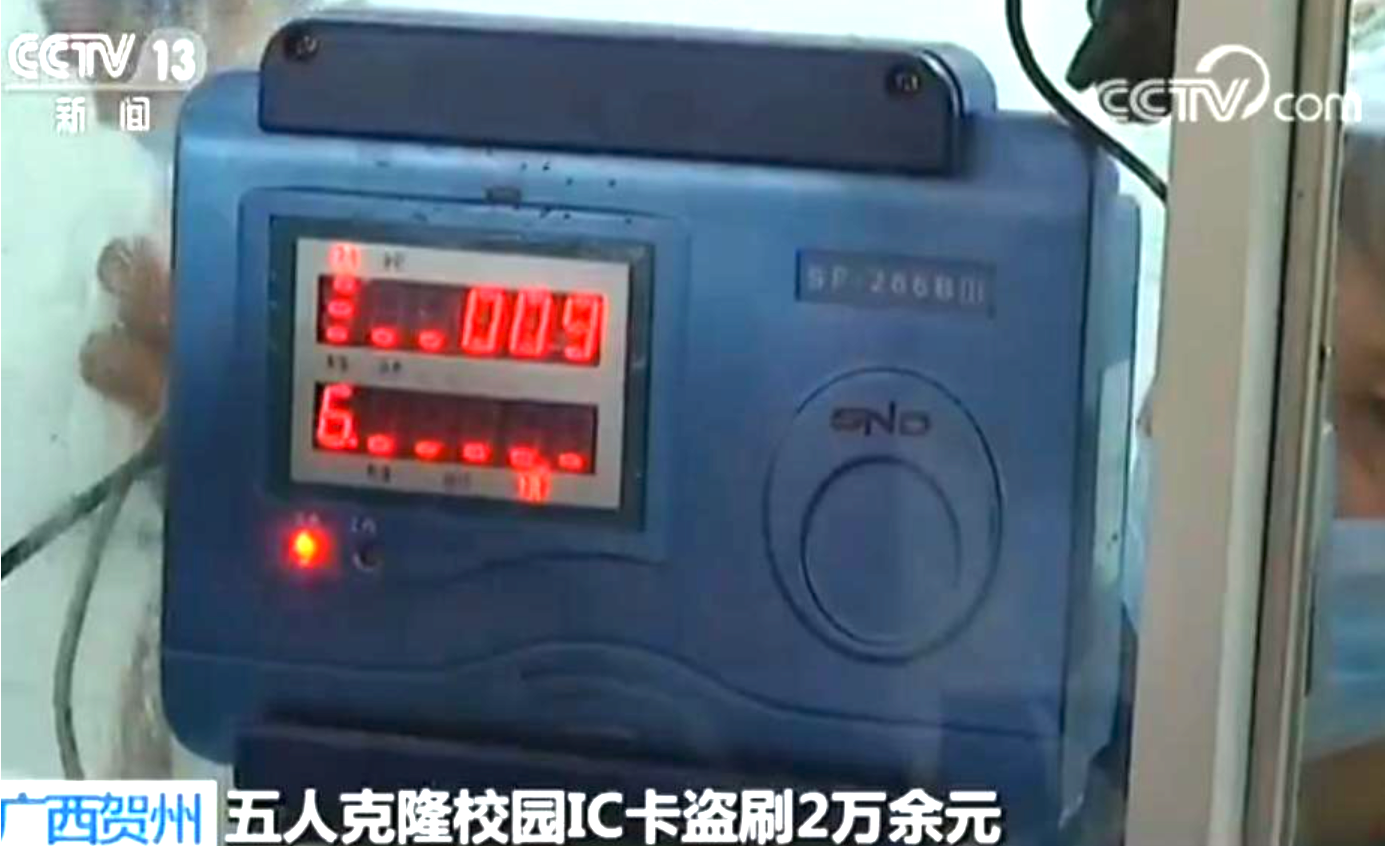
\includegraphics[width=0.75\textwidth]{figures/M1card.png}
	\caption{广西贺州未成年人克隆校园IC卡盗刷案新闻报道}
	\label{fig:case1_school}
\end{figure}

\textbf{案例二：全球酒店门锁“Unsaflok”漏洞}

dormakaba官方承认，Saflok系统存在与门卡底层数据保护相关的漏洞（CVE-2024-29916）：攻击者只要拿到任意一张有效或过期的房卡，就可能伪造门卡，打开该物业内的任意房门。这一漏洞\textbf{影响到131个国家超过1.3万处物业的300多万扇门}。

这两个典型案例一内一外构成完整链路：一旦门禁底层算法和凭证体系有结构性漏洞，影响就不再是一张卡、一个门，而可能是一整栋楼、一整家酒店，甚至\textbf{一个完整的物业系统}。

\section{M1卡的代价不是“便宜”，而是“昂贵”}

物业和开发商选择M1卡的唯一理由是“便宜”（单卡几毛钱）。但实际上，真正被忽视的是巨大的\textbf{后续成本（TCO）}：事故处置、系统补洞、运维返工、用户投诉以及最难修复的\textbf{信任损失}。门禁一旦被证明“可以复制”，它就沦为了一个迟早出事的摆设。

在法律层面，已有大量判例显示，因门禁卡漏洞导致业主失窃，\textbf{物业需承担20\%到50\%的赔偿责任}，单次赔偿达数万至十几万元。一个千户小区一次入室盗窃的赔偿金额，就已经远超全小区门禁卡升级的全部成本。看似省了几块钱，实则是赌上了业主的安全与物业的巨额赔偿。
	% ==========================================
% 第二章
% ==========================================
\chapter{一场无法回避的风暴——量子计算威胁与全球响应}

\section{CPU卡：今天安全，明天过时}

很多人认为，换成CPU卡就安全了。但残酷的现实是：\textbf{CPU卡只能解决当下的安全问题，在即将到来的量子计算时代，它和M1卡一样不堪一击。}

目前主流的国密CPU卡，安全核心依赖SM2（ECC-256）公钥密码算法。而量子计算机的\textbf{Shor算法}，仅需约1500个逻辑量子比特，就能\textbf{彻底攻破 ECC-256 算法}；\textbf{Grover算法}则会让对称加密的安全强度直接减半（如SM1/SM7直接降至64bit）。

只要门禁的核心仍建立在ECC一类算法之上，它就只是\textbf{“在量子时代到来前暂时安全”}。现在花大价钱升级传统CPU卡，不过是从一个已经破了的洞，跳进了一个几年后一定会破的洞。

\begin{table}[htbp]
	\centering
	\caption{全代际门禁卡量子安全评估}
	\label{tab:quantum_assessment}
	\renewcommand{\arraystretch}{1.2} % 稍微增加行高，使表格更美观
	\begin{tabular}{llccr}
		\toprule
		\textbf{卡类型} & \textbf{加密算法} & \textbf{当前安全性} & \textbf{量子计算下} & \textbf{单卡成本} \\
		\midrule
		ID卡 & 无 & $\times$ 零安全 & $\times$ 不安全 & $\sim$0.2元 \\
		M1卡 & Crypto-1 (48bit) & $\times$ 已全面破解 & $\times$ 不安全 & $\sim$0.5-1元 \\
		MIFARE Plus & AES-128 & $\checkmark$ 相对安全 & $\triangle$ 降级至64bit & $\sim$2-5元 \\
		MIFARE DESFire & 3DES/AES + ECC & $\checkmark$ EAL4+ & \textbf{$\times$ ECC被破解} & $\sim$5-15元 \\
		MIFARE DUOX & AES-256 + ECC-256 & $\checkmark\checkmark$ 当前最强 & \textbf{$\times$ ECC被破解} & $\sim$10-20元 \\
		CPU卡(国密) & SM1/SM7 + SM2(ECC) & $\checkmark\checkmark$ 金融级 & \textbf{$\times$ SM2被破解} & $\sim$5-15元 \\
		\bottomrule
	\end{tabular}
\end{table}

\section{Q-Day不是“如果”，而是“何时”}

量子计算机破解经典密码体系的那一天被称为 \textbf{Q-Day}。Gartner预测，ECC算法在\textbf{2029年就会变得不安全}。破解ECC所需的量子比特预估，从2012年的10亿个降至2025年的100万个，六年下降95\%！中国科学家也已对主流加密方法发起了世界上第一个有效的量子攻击。

更可怕的是，量子威胁不是等Q-Day到来才出现。目前，国家级对手和黑客组织正在大规模执行\textbf{“先收集，后解密”（Store Now, Decrypt Later）}策略。门禁出入记录包含人员、时间、区域活动模式，是极高价值的情报。对政府、军工、金融等关键基础设施而言，今天的门禁数据，已经在为明天的量子攻击备货。

\section{全球已拉响警报}

后量子密码（PQC）迁移已成为全球共识：
\begin{itemize}
	\item \textbf{美国NIST}：2024年8月发布首批后量子密码标准，明确2030年全面弃用、\textbf{2035年完全禁用RSA与ECC算法}。
	\item \textbf{美国国防部CNSA 2.0}：要求\textbf{2025年起}，后量子密码必须作为默认加密算法。
	\item \textbf{科技巨头入局}：IBM、微软成立联盟，谷歌Chrome已集成抗量子加密。
	\item \textbf{中国产业动态}：2025年2月，国家商用密码标准研究院全面启动抗量子商用密码算法征集；第三代“本源悟空”装备国内首个后量子密码护盾。
\end{itemize}

资本市场同样反应热烈：2024年全球后量子密码市场估值1.79亿美元，预计2031年将达22亿美元（CAGR 43.1\%），其中\textbf{量子安全认证解决方案是增速最快的子领域}。

\section{等不起——Mosca定理与迁移窗口}

历史经验表明，一项密码算法从标准化到完全融入系统完成落地，普遍需要10到20年。密码学界著名的 \textbf{Mosca定理（莫斯卡定理）} 为我们划下了红线：

\begin{center}
	\textbf{数据保护年限 (X) + 系统迁移时间 (Y) > 量子计算机建成时间 (Z) $\Longrightarrow$ 必须立刻行动！}
\end{center}

我们的门禁系统需要保障未来10年的安全，全行业完成PQC迁移至少需要5-10年，而量子计算机预计10年内就会攻破现有体系。正如Gartner副总裁警告：“等到接近2030年才采取行动的组织，将没有足够的时间完成安全替换。”

如果现在不启动迁移，当Q-Day到来时我们将毫无还手之力。而我们自主研发的 \textbf{基于 PQ-Aliro 协议的后量子门禁系统}，正是解决这一痛点的终极解：\textbf{一步到位完成量子安全升级，守住当下的门，更守住未来的安全。}
	% ==========================================
% 第二篇 导入过场页
% ==========================================
\cleardoublepage
\thispagestyle{empty} % 让过场页干干净净，没有页眉页脚

\vspace*{6cm} % 整体垂直向下偏移，营造留白的高级感

\begin{center}
	% 篇章标题
	{\heiti\erhao 第二篇\quad 我们创造了什么} 
	\addcontentsline{toc}{part}{第二篇\quad 我们创造了什么}
	
	\vspace{2cm} % 标题与文案之间的间距
	
	% 灵魂文案
	{\songti\xiaosi \textit{“这不是卖一张更贵的卡，而是定义一个品类；\\ [0.5em] 这不是做一次交易，而是构建一个面向未来二十年的物理安全生态。”}}
\end{center}

\vfill
\cleardoublepage % 过场页结束，下一页正式开始第三章正文


% ==========================================
% 第三章
% ==========================================
\chapter{产品与技术方案}

\section{产品架构总览}

本方案针对通用门禁场景在量子计算时代面临的核心安全风险，构建了\textbf{“芯片-卡片-终端-平台”全链路抗量子安全架构}。依托团队在\textbf{武汉大学密码学与区块链实验室}的深厚技术积累，以自主研发的高性能后量子密码（PQC）算法库为核心底座，自上而下分为卡片层、读卡器层、后台层三个核心层级，实现端到端量子安全防护，同时完全兼容现有门禁系统，支持存量系统的平滑迁移。

本架构的核心设计原则包括：
\begin{enumerate}
	\item \textbf{全链路抗量子安全}：所有核心身份认证、密钥协商环节均采用NIST标准化的PQC算法，彻底抵御Shor算法对ECC/SM2的破解风险。
	\item \textbf{密码敏捷性设计}：底层算法栈支持热切换与动态升级，可快速适配未来标准与国密后量子算法，避免硬件替换成本。
	\item \textbf{全场景兼容适配}：向下兼容ISO 14443/15693、M1卡、国密CPU卡等现有生态，实现无感化后量子升级。
	\item \textbf{高性能低功耗优化}：针对门禁无源卡片、低功耗特性，对核心算法进行硬件与工程级深度优化，满足非接触式毫秒级响应。
\end{enumerate}

\begin{table}[htbp]
	\centering
	\caption{整体架构与核心技术能力}
	\renewcommand{\arraystretch}{1.3}
	\begin{tabular}{cp{4.5cm}p{4cm}p{5cm}}
		\toprule
		\textbf{层级} & \textbf{核心产品} & \textbf{核心能力} & \textbf{底层技术支撑} \\
		\midrule
		\textbf{卡片层} & PQC门禁卡 \newline (内置自主PQC安全SE芯片) & 后量子身份认证、双向密钥协商、凭证安全存储 & ML-KEM密钥封装、ML-DSA签名、国密算法、混合密钥推导 \\
		\textbf{读卡器层} & PQC门禁读卡器 \newline + PQC-SAM安全模块 & PQC协议解析处理、双向身份认证、OTA升级 & 嵌入式PQC算法优化、SAM硬件隔离、固件验签 \\
		\textbf{后台层} & 量子安全密钥管理平台 \newline (Quantum-Safe KMS) & 密钥全生命周期管理、密码敏捷性引擎、安全监控 & 分布式密钥存储、算法热切换、国密合规与等保适配 \\
		\bottomrule
	\end{tabular}
\end{table}

本架构的技术底座采用创新的\textbf{四层解耦合架构}设计，可实现跨芯片、跨终端的无缝适配：
\begin{itemize}
	\item \textbf{基础算子层}：提供有限域运算、矩阵向量乘加、大数运算等统一底层算力。
	\item \textbf{多项式运算层}：集成深度优化的NTT/INTT变换、多项式采样与规约算法。
	\item \textbf{哈希函数与采样层}：提供Keccak海绵结构、SHAKE可扩展输出及高斯/均匀采样。
	\item \textbf{算法实现与协议层}：拼装实现ML-KEM/ML-DSA等标准算法，并面向门禁场景提供APDU指令与认证协议集。
\end{itemize}

如下页图所示，通过高复用的底层算子设计，我们的代码体积明显减小，更好适配门禁卡此类嵌入式场景。
\begin{figure}
	\centering
	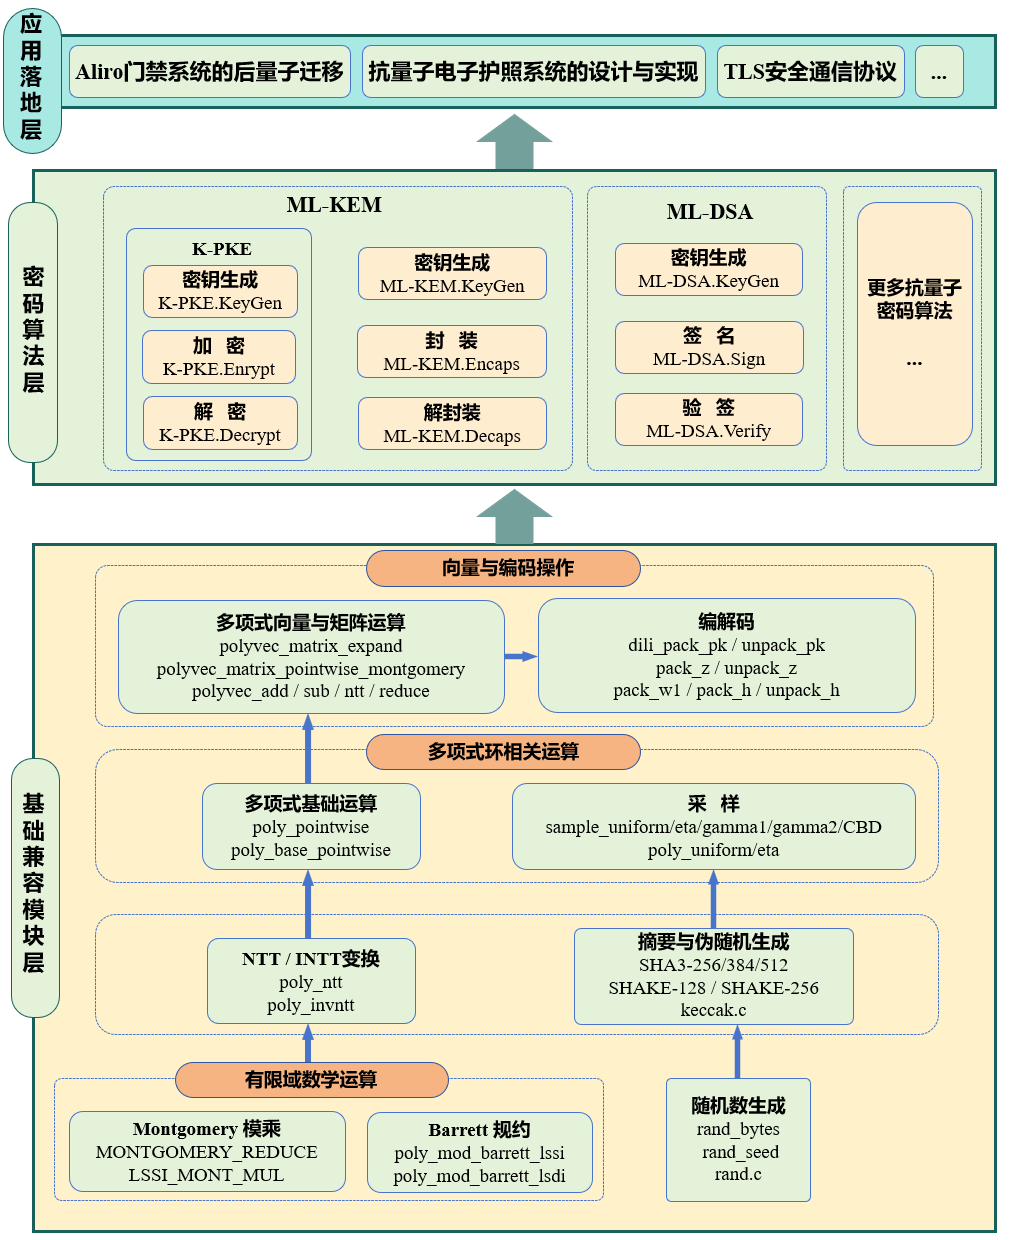
\includegraphics[width = \textwidth ]{figures/structures.png}
	
\end{figure}

\section{芯片层：PQC安全元件（SE）}

PQC安全元件是本方案的核心硬件信任根，专为门禁低功耗、高安全需求设计，是国内首款针对门禁场景优化的软硬协同抗量子安全芯片。\textbf{目前团队已与汇鼎科技等头部芯片厂商达成初步合作意向}，正推进PQC算法在物联网SE芯片上的流片与适配验证。

\subsection{芯片核心硬件架构}

采用“安全核+PQC协处理器+存储控制+通信接口”的四级架构：
\begin{enumerate}
	\item \textbf{32位安全主控核}：采用符合国密二级要求的RISC-V内核，内置硬件TRNG，支持内存隔离，密钥明文永不暴露到隔离区外。
	\item \textbf{专用PQC硬件协处理器}：针对格密码设计专用流水线，内置NTT加速单元与蒙哥马利模乘单元，运算速度比纯软件提升17倍以上。
	\item \textbf{国密算法硬件引擎}：内置SM1/SM4/SM7/SM2/SM3加速模块，与PQC引擎共享资源，实现双体系并行。
	\item \textbf{安全存储单元}：内置eFlash/ROM，支持防篡改、防物理攻击，密钥不可导出。
	\item \textbf{非接触式通信接口}：支持NFC无源模式（最高424kbps），针对PQC大尺寸密文优化通信帧结构，降低交互耗时。
\end{enumerate}

\subsection{内置PQC算法栈与底层数学实现}

\subsubsection{核心支持算法清单}

\begin{table}[htbp]
	\centering
	\caption{SE芯片内置核心支持算法}
	\renewcommand{\arraystretch}{1.2}
	\begin{tabular}{lllp{5.5cm}}
		\toprule
		\textbf{算法类别} & \textbf{算法名称} & \textbf{标准合规性} & \textbf{核心应用场景} \\
		\midrule
		抗量子密钥封装 & ML-KEM 512/768 & NIST FIPS 203 & 门禁双向密钥协商、会话密钥生成 \\
		抗量子数字签名 & ML-DSA 44/65 & NIST FIPS 204 & 门禁卡身份认证、固件签名验签 \\
		抗量子哈希签名 & SLH-DSA & NIST FIPS 205 & 根证书签名、长期身份凭证签名 \\
		国密对称算法 & SM1/SM4/SM7 & GM/T 0001-2012 & 门禁数据端到端加密、卡片存储加密 \\
		国密公钥算法 & SM2 & GM/T 0003-2012 & 兼容现有国密门禁、双算法混合认证 \\
		国密哈希算法 & SM3 & GM/T 0004-2012 & 数据摘要、挑战值生成、哈希绑定 \\
		\bottomrule
	\end{tabular}
\end{table}

\subsubsection{底层数学运算优化}

芯片内置算法库严格遵循格密码数学理论，针对无源低功耗场景做了深度定向优化：
\begin{enumerate}
	\item \textbf{多项式环运算}：基于商环 $\mathcal{R}_q=\mathbb{Z}_q[X]/(X^n+1)$ 构建核心运算。针对ML-KEM ($q=3329, n=256$) 和 ML-DSA ($q=8380417, n=256$)，采用负循环卷积实现多项式乘法，将复杂度从 $\mathcal{O}(n^2)$ 降至 $\mathcal{O}(n\log n)$。
	\item \textbf{数论变换（NTT）加速}：内置Cooley-Tukey正向NTT与GS逆向NTT硬件流水线。针对ML-KEM参数特性，优化了二次模乘的基乘运算，解决了512次本原单位根缺失带来的复杂度问题。
	\item \textbf{模约简算法优化}：集成Montgomery与Barrett双模约简。Montgomery用于NTT蝶形运算，引入基 $R=2^{32}$ 将模乘转化为移位与乘加；Barrett约简用于实现\textbf{常数时间执行}，抵御时序侧信道攻击。
	\item \textbf{采样算法实现}：内置CBD（中心二项分布）等专用采样，基于SHAKE进行伪随机数扩展，严格消除侧信道泄露风险。
	\item \textbf{紧凑编解码模块}：针对公钥和密文设计紧凑编码，序列化公钥长度压缩至 $32 + k \times 384$ 字节，大幅降低非接触式通信开销。
\end{enumerate}

\subsubsection{算法性能对标}

与业内主流开源PQC库（如PQ-magic）相比，本方案在门禁受限环境中实现了显著的性能跃升：

\begin{table}[htbp]
	\centering
	\caption{核心算法性能对标（基于相近主频MCU环境）}
	\renewcommand{\arraystretch}{1.2}
	\begin{tabular}{lccc}
		\toprule
		\textbf{算法/操作} & \textbf{本方案 (时钟周期)} & \textbf{业内开源库 (时钟周期)} & \textbf{性能提升} \\
		\midrule
		ML-DSA-44 密钥生成 & 233,121 & 586,151 & \textbf{+60.2\%} \\
		ML-DSA-44 签名验证 & 247,464 & 546,125 & \textbf{+54.7\%} \\
		ML-DSA-65 密钥生成 & 435,309 & 1,066,442 & \textbf{+59.2\%} \\
		ML-DSA-65 签名验证 & 488,229 & 925,238 & \textbf{+47.2\%} \\
		\bottomrule
	\end{tabular}
\end{table}

\subsection{安全防护与合规设计}
本方案具备\textbf{硬件级防侧信道攻击机制}（支持掩码防护、电磁屏蔽、时序混淆）、\textbf{硬件防火墙隔离机制}，设计符合《商用密码产品认证规则》，可支持国密二级与EAL5+安全认证。

\section{卡片层：后量子门禁卡}

\subsection{物理与通信规格}
完全符合 ISO 7816 ID-1 标准，支持定制封装。兼容 ISO 14443 A/B 和 ISO 15693 协议，无源模式读卡距离 $\ge$ 5cm，\textbf{单次完整认证流程耗时 $\le$ 300ms}，满足快通行需求。

\subsection{核心安全机制}

\textbf{1. 经典+PQC混合认证模式} \\
为平衡前瞻性与兼容性，采用“SM2/AES+ML-DSA/ML-KEM”\textbf{双轨并行认证}。两路认证独立执行、结果并行校验，单侧算法失效不影响整体安全边界。

\textbf{2. 混合密钥推导机制} \\
独立生成传统会话密钥 $K_1$ 与抗量子会话密钥 $K_2$，通过标准化HKDF函数进行绑定派生：
\[ K_{final} = \text{HKDF}(\text{SHA3-512}, K_1 \parallel K_2) \]
该机制彻底杜绝了单算法被攻破导致的会话密钥泄露风险。

\textbf{3. 防克隆与一次一密} \\
卡内密钥与SE芯片序列号\textbf{硬件绑定}，不可被克隆至其他芯片；每次刷卡通过双重随机挑战值（Challenge）派生全新密钥，确保刷卡数据\textbf{一次一密}，彻底杜绝嗅探与重放攻击。

\subsection{卡内APDU指令集实现}
卡片内置完整的扩展APDU指令集，不仅支持 `0x84` 获取传统挑战值、`0x82` 外部认证，更针对PQC协议增加了后量子专用指令族（如 `CLA=0x80`, `INS=0xB1` 获取PQC公钥，`0xB2` ML-KEM密钥封装等），完全兼容 ISO 7816-4 规范。

\section{读卡器层：PQC门禁读卡器}

读卡器内置 \textbf{PQC-SAM安全模块}，支持PQC协议终端侧处理及多协议向下兼容（M1卡/国密CPU卡）。

\subsection{核心功能与技术实现}

\begin{itemize}
	\item \textbf{多协议并行认证引擎}：自动识别卡片类型匹配协议。针对混合认证卡片，并行执行双链路认证而不增加额外耗时。
	\item \textbf{OTA安全固件升级}：采用 ML-DSA+SM2 \textbf{双算法固件验签}，A/B双分区防变砖设计，杜绝供应链攻击与恶意固件刷入。
	\item \textbf{抗量子认证协议 (PQ-Aliro)}：采用2-RTT两轮往返交互模式。第一阶段利用 ML-KEM 进行临时密钥交换；第二阶段使用 ML-DSA 进行双向签名认证与上下文哈希绑定。在不增加交互轮次的前提下完成强身份认证。
\end{itemize}

\subsection{嵌入式算法优化 (非公平优势体现)}
在MCU资源受限环境下，团队利用四层解耦合架构实现了极限优化：
\begin{enumerate}
	\item \textbf{深度代码复用}：ML-KEM与ML-DSA\textbf{完全复用底层的NTT模块}、多项式运算与哈希模块，大幅压缩固件体积，Flash占用减少超35KB。
	\item \textbf{流式哈希处理}：引入 Init-Update-Final 模式，无需将长报文一次性读入RAM，峰值内存占用降低60\%。
	\item \textbf{零拷贝数据处理}：算法直接操作通信缓冲区指针进行原地位解码，内存搬运延迟降低40\%。
\end{enumerate}

\section{后台层：量子安全密钥管理平台}

平台（Quantum-Safe KMS）采用微服务架构，分为接入层、服务层、数据层。为全系统提供统一的密码服务能力。

\begin{itemize}
	\item \textbf{密钥全生命周期管理}：依托硬件密码机生成真随机数，实现PQC与国密密钥的批量生成、安全分发、自动轮换与合规销毁。
	\item \textbf{密码敏捷性引擎 (Crypto-Agility)}：全算法采用插件化封装。支持算法版本、参数的\textbf{在线热切换}与灰度升级，无需更换底层硬件即可应对未来密码标准的演进。
	\item \textbf{智能安全监控}：基于规则引擎与机器学习识别异常刷卡（如高频、异地、防重放探测），自动触发设备锁定，并生成不可篡改的区块链审计日志。
\end{itemize}

\section{与现有最高端产品的全面对比}

本方案相较于当前业内最高端的高频门禁卡（MIFARE DESFire、国密SM2 CPU卡），在安全前瞻性与底层机制上实现了代际跨越：

\begin{table}[htbp]
	\centering
	\caption{门禁核心技术能力代际对比}
	\label{tab:comparison}
	\renewcommand{\arraystretch}{1.3}
	\small
	\begin{tabular}{p{2cm}p{3.5cm}p{3.5cm}p{5cm}}
		\toprule
		\textbf{能力维度} & \textbf{MIFARE DESFire} & \textbf{国密 CPU卡} & \textbf{本方案：后量子门禁卡} \\
		\midrule
		\textbf{公钥认证} & ECC-256 (\textbf{量子不安全}，可被Shor算法破解) & SM2 (\textbf{量子不安全}，可被Shor算法破解) & \textbf{ML-DSA} (NIST标准抗量子算法，量子安全) \\
		\textbf{密钥协商} & ECDH (\textbf{量子不安全}) & SM2 密钥协商 & \textbf{ML-KEM} (NIST抗量子密钥封装) \\
		\textbf{防克隆机制} & UID+AES 加密防护 & CPU芯片+国密算法 & \textbf{PQC+国密双重认证}，硬件根信任深度绑定 \\
		\textbf{合规前瞻性} & 不满足2030+抗量子要求 & 不满足2030+抗量子要求 & \textbf{符合NIST最新标准}，预留国密后量子演进接口 \\
		\textbf{密码敏捷性} & 固定算法栈，升级需换卡 & 固定算法栈，升级需换卡 & \textbf{底层算子解耦，算法可热更新} \\
		\textbf{侧信道防护} & 基础防护，无针对性设计 & 硬件级防护 & 硬件掩码+时序混淆+核心算法\textbf{常数时间执行} \\
		\textbf{协议交互} & 2-RTT单算法认证 & 2-RTT单算法认证 & \textbf{2-RTT双算法并行认证}，不增加额外耗时 \\
		\textbf{认证耗时} & ECC验签约 1.2ms & SM2验签约 1.5ms & \textbf{软硬协同优化 $\le$ 5ms}，满足门禁极速响应体验 \\
		\bottomrule
	\end{tabular}
\end{table}

	% ==========================================
% 第三篇 导入过场页
% ==========================================
\cleardoublepage
\thispagestyle{empty} % 让过场页干干净净，没有页眉页脚

\vspace*{6cm} % 整体垂直向下偏移，营造留白的高级感

\begin{center}
	% 篇章标题
	{\heiti\erhao 第三篇\quad 我们改变了什么} 
	\addcontentsline{toc}{part}{第三篇\quad 我们改变了什么}
	
	\vspace{2cm} % 标题与文案之间的间距
	
	% 灵魂文案
	{\songti\xiaosi \textit{“不是卖一张卡片，而是定义一个品类；\\ [0.5em] 不是做一次交易，而是构建一个生态。”}}
\end{center}

\vfill
\cleardoublepage % 过场页结束，下一页正式开始第六章正文

% ==========================================
% 第四章
% ==========================================
\chapter{目标客户与商业落地}

\section{市场需求：以NFC贴片切入的“降维打击”}

本项目以PQ-Aliro智慧门禁系统为总体方向，但在商业落地上，直接从整套高门槛门禁系统入手面临极高的决策阻力。经过深度调研，我们选择以\textbf{NFC安全增强贴片}作为切入口来推进整个项目的规模化。

从行业发展环境看，NFC技术在短距离通信场景中具有明显优势。随着数字经济的发展，央行数据显示2025年一季度移动支付金额达152.64万亿元，“碰一碰”模式持续强化了用户对非接触式交互的接受度。据行业调研数据，\textbf{2024年中国近场通信（NFC）行业市场规模约为925亿元，同比增长21.72\%}。

当前NFC贴片已经广泛应用于门禁、身份识别等场景，但其安全能力长期被忽视。市场上大量NFC贴片仅承担“触发”功能，缺乏高强度加密保护，面临极高的复制与伪造风险。这种\textbf{“普及在前、安全滞后”}的状态，使得NFC贴片领域天然存在明确的安全升级刚需。

这一需求之所以值得作为商业突破口，在于它同时具备三个核心特点：
\begin{itemize}
	\item \textbf{需求基础广泛}：NFC贴片价格低、适配性强，已渗透到海量日常场景。安全痛点一旦被平价解决，将释放出极其庞大的市场空间。
	\item \textbf{替换门槛极低}：与整套门禁系统替换相比，贴片级安全增强更贴近现有使用习惯，不增加企业的部署负担，极易被市场快速接受。
	\item \textbf{具备自然延展性}：贴片是物理入口，其背后连接着完整的身份认证链路。一旦贴片侧的安全能力被认可，项目就有条件顺理成章地向终端读卡器、后台KMS平台乃至整套安防系统的升级延展。
\end{itemize}

因此，我们面对的并非一个需要从零教育的全新市场，而是一个\textbf{已经存在、正在扩张、且急需安全赋能}的存量蓝海。

\section{目标客户分层}

基于上述市场需求，本项目的目标客户分为C端、B端和G端三个层级。三者并非并列关系，而是对应着项目\textbf{不同生命周期阶段的市场价值}。

\begin{itemize}
	\item \textbf{C端（广度验证池）}：最广泛、最易切入的起步市场。核心价值在于用户基数大、反馈极快。能帮助项目快速验证“PQC贴片”的可用性，并在早期形成高周转的稳定现金流。
	\item \textbf{B端（利润复制盘）}：项目从单点走向系统化落地的关键市场。园区、企业总部等B端客户不再仅关注单一硬件，而是看重系统的兼容性与整体改造成本。这是项目从“消费级安全”走向“组织级方案”的重要承接层。
	\item \textbf{G端（价值制高点）}：商业化路径中的高价值市场。政府机关、重点公共设施对成熟度、可审计性要求极高。G端不作为最初切入点，而是项目跑通模式后，建立品牌信任背书与获取高溢价的终极目标。
\end{itemize}

\begin{table}[htbp]
	\centering
	\caption{目标客户分层与核心逻辑}
	\label{tab:customer_segments}
	\renewcommand{\arraystretch}{1.4}
	\begin{tabular}{p{1.5cm}p{3.5cm}p{4cm}p{4.5cm}}
		\toprule
		\textbf{客户层级} & \textbf{典型场景} & \textbf{核心需求} & \textbf{商业市场价值} \\
		\midrule
		\textbf{C端} & 广泛个人与轻量化NFC应用场景 & 低成本、安全增强、便捷部署 & 易推广、反馈快、形成初期高周转现金流 \\
		\midrule
		\textbf{B端} & 园区、楼宇、企业总部、教育医疗机构 & 系统兼容、安全升级、降低总改造成本 & 摆脱价格战，推动标准化复制，形成系统化收入 \\
		\midrule
		\textbf{G端} & 政府机关、重点公共设施、高敏感场景 & 高可信、高稳定、可审计、长期绝对安全 & 形成高价值标杆，获取溢价与国家级品牌背书 \\
		\bottomrule
	\end{tabular}
\end{table}

\section{市场路径与商业模式}

本项目的商业演进遵循统一的底层逻辑：从轻量级贴片切入，通过逐步提升产品形态和服务深度，最终形成\textbf{可持续的SaaS与服务盈利结构}。

\begin{enumerate}
	\item \textbf{第一阶段：C端验证期（产品型模式）} \\
	采取“低门槛切入、快速铺量”策略。以NFC安全增强贴片为核心产品，收入主要来源于硬件销售。核心目标是占领入口、获取反馈、支撑后续研发。
	\item \textbf{第二阶段：B端复制期（方案型模式）} \\
	采取“方案整合、标准复制”策略。将单一贴片升级为“贴片凭证+终端读卡器+认证模组+后台”的整体门禁安全方案。收入扩展为\textbf{硬件+项目实施+平台服务}，核心目标是提升客单价。
	\item \textbf{第三阶段：G端提升期（平台型模式）} \\
	采取“成熟切入、案例驱动”策略。项目价值向\textbf{持续服务能力}转移，通过KMS密钥管理、OTA软件升级、系统巡检等，形成高壁垒的年度运维收入，极大延长客户生命周期价值（LTV）。
\end{enumerate}

\begin{table}[htbp]
	\centering
	\caption{市场路径与商业模式三阶段演进}
	\label{tab:business_phases}
	\renewcommand{\arraystretch}{1.4}
	\begin{tabular}{cp{1.5cm}p{3cm}cp{3.5cm}p{3cm}}
		\toprule
		\textbf{阶段} & \textbf{目标市场} & \textbf{市场拓展策略} & \textbf{商业形态} & \textbf{核心收入结构} & \textbf{战略目标} \\
		\midrule
		\textbf{第一阶段} & C端 & 低门槛切入、快速铺量 & \textbf{产品型} & 硬件销售收入 & 验证产品，形成初期现金流 \\
		\textbf{第二阶段} & B端 & 方案整合、标准化复制 & \textbf{方案型} & 硬件 + 实施 + 平台服务收入 & 提升客单价，形成标准化交付 \\
		\textbf{第三阶段} & G端 & 成熟体系切入、案例驱动 & \textbf{平台型} & 平台SaaS服务 + 长期运维收入 & 建立可持续收益与合规高壁垒 \\
		\bottomrule
	\end{tabular}
\end{table}

\section{定价方式：动态匹配产品生命周期}

在定价策略上，项目摒弃了一成不变的硬件加价率模型，而是基于客户所处阶段的“核心价值关注点”进行动态升维：

\begin{itemize}
	\item \textbf{C端（低门槛渗透定价）}：NFC贴片本身边际成本低，具备极大操作空间。我们将以\textbf{极度友好的价格}快速占领场景，不强求单件高毛利，而是依靠高渗透和高周转获取市场基数。
	\item \textbf{B端（综合方案定价）}：B端客户购买的是“安全改造包裹”。定价将围绕硬件、终端适配和SaaS服务综合展开。通过锚定\textbf{更低的总拥有成本（TCO）}，摆脱单一贴片的价格战，依靠整体方案支撑更高的毛利空间。
	\item \textbf{G端（安全合规溢价）}：政企客户对价格的敏感度远低于对“政治正确与绝对安全”的关注。定价将深度绑定国家密码合规标准，依靠成熟的交付资质和长期服务能力，收取丰厚的\textbf{高可信安全溢价}。
\end{itemize}

\begin{table}[htbp]
	\centering
	\caption{分阶段与分客群的定价逻辑}
	\label{tab:pricing_strategy}
	\renewcommand{\arraystretch}{1.4}
	\begin{tabular}{cp{3cm}p{4cm}p{5.5cm}}
		\toprule
		\textbf{客户层级} & \textbf{核心定价逻辑} & \textbf{客户关注点 (痛点)} & \textbf{项目盈利方式} \\
		\midrule
		\textbf{C端} & 低门槛、高渗透定价 & 价格友好、极易尝试与部署 & 通过高周转与规模化硬件销量获取早期现金 \\
		\midrule
		\textbf{B端} & 整体方案定价 & 改造的整体价值、总拥有成本 (TCO) & 摆脱单品价格战，以综合服务支撑更高客单价 \\
		\midrule
		\textbf{G端} & 安全与合规溢价 & 系统稳定性、可审计性、长效运维能力 & 依托资质背书，签署高价值年度服务合同 (SaaS) \\
		\bottomrule
	\end{tabular}
\end{table}
	% ==========================================
% 第五章
% ==========================================
\chapter{竞品分析与经济性论证}

\section{物理安防领域的PQC空白}

\subsection{传统门禁卡市场的安全困境}

当前物理访问控制市场仍以传统加密技术为主导。根据行业数据，2023年全球门禁卡出货量超过8亿张，其中\textbf{约65\%仍在使用 MIFARE Classic（M1）等存在已知漏洞的技术}。M1卡采用的 Crypto-1 算法早在2008年被完全破解，使用价值百美元的设备即可在数秒内克隆卡片。

\begin{table}[htbp]
	\centering
	\caption{主流门禁技术安全性与成本对比（2023年）}
	\label{tab:market_tech_comparison}
	\renewcommand{\arraystretch}{1.3}
	\begin{tabular}{p{2.5cm}p{3cm}cp{3cm}cp{1.5cm}}
		\toprule
		\textbf{技术类型} & \textbf{典型代表} & \textbf{量子安全} & \textbf{破解成本} & \textbf{单卡成本} & \textbf{市场份额} \\
		\midrule
		\textbf{低频 ID卡} & EM4100 & 否 & 50元设备 & 0.5-1元 & 15\% \\
		\textbf{MIFARE} & M1卡 & 否 & 100元设备 & 1-3元 & \textbf{65\%} \\
		\textbf{CPU卡} & DESFire / 国产SM系列 & 部分抗量子 & 数万元设备 & 5-15元 & 18\% \\
		\textbf{生物识别} & 人脸/指纹 & 是 & 物理仿冒 & 3000-10000元 & 2\% \\
		\midrule
		\textbf{PQC产品} & \textbf{本项目 (贴片/卡)} & \textbf{是} & \textbf{需百万级量子比特} & \textbf{20-30元} & \textbf{<0.1\%} \\
		\bottomrule
	\end{tabular}
\end{table}

\subsection{现有PQC厂商的局限性}

尽管后量子密码学已成为研究热点，但市场应用仍局限于特定领域，物理安防层存在巨大空白：
\begin{itemize}
	\item \textbf{云端通信与数字证书}：PQShield 专注于IP核和软件库，缺乏物理层集成经验；IBM 提供量子安全TLS服务，主要面向云服务商，单证书年费高达数百美元。
	\item \textbf{区块链与数字货币}：如 QANplatform 为首个抗量子区块链平台，但专注于数字资产保护，未涉及物理访问控制。
	\item \textbf{传统安防厂商的滞后}：作为 MIFARE 技术持有者，NXP 的路线图显示 PQC 产品计划在2026年后推出；海康威视/大华等巨头当前精力集中于视频监控AI化，门禁仍采用传统 CPU 卡方案。
\end{itemize}

\subsection{竞争窗口期分析}

基于以下关键时间节点，物理安防领域的 \textbf{PQC 竞争窗口期约为 3-5 年}：
\begin{enumerate}
	\item \textbf{标准制定进程}：NIST 已于2024年正式发布 FIPS 203/204/205 标准；中国密标委预计2025年发布后量子密码算法系列国标。
	\item \textbf{强制迁移时间表}：美国CNSA 2.0 要求\textbf{2030年前}完成向 PQC 迁移；欧盟建议关键基础设施在\textbf{2027年前}启动升级。
	\item \textbf{产业链成熟度}：目前尚无专为门禁优化的 PQC 芯片量产，现有方案多为 FPGA 或纯软件实现，成本过高。我们的“PQC近场通信贴片”方案恰好切入了这一蓝海。
\end{enumerate}

\section{TCO模型下的竞争优势}

业界普遍预测，2030年前后各国政府将强制要求淘汰旧有密码标准。在这个历史过渡期，我们引入\textbf{总拥有成本（TCO）}核心概念，论证为何一步到位升级 PQC 是最经济的选择。

\subsection{传统升级路径的隐性成本}

\textbf{【核心假设说明】}
\begin{itemize}
	\item \textbf{软性成本占比}：参考 Gartner 调研，传统安防集成项目中，硬件采购仅占 30\%，而\textbf{施工、调试、培训、数据迁移等软性开销占 70\%}。
	\item \textbf{停机成本}：保守估算，1000人园区因系统切换导致的生产效率损失、安保漏洞等，按 5万元/天 计算，停机 3 天。
	\item \textbf{生命周期}：传统 CPU 卡因面临量子破解威胁，有效生命周期仅剩约 5 年（至2030年）；而 PQC 贴片技术前瞻，生命周期可视为 10 年。
\end{itemize}

以拥有 1000 个门禁点的大型园区为例，对比两种升级路径：

\vspace{0.5em}
\noindent\textbf{方案 A（分步升级）：传统 CPU 卡 $\rightarrow$ 未来 PQC}
\begin{itemize}
	\item \textbf{第 0 年（第一次升级：部署 CPU 卡系统）}：硬件成本 6.5万元；软性成本（按70\%核算）约 15.1万元。第一次总投入：\textbf{21.6万元}。
	\item \textbf{第 5 年（第二次升级：替换为 PQC 系统）}：硬件成本 6.0万元；软性成本约 14.0万元；停机损失 15.0万元。第二次总投入：\textbf{35.0万元}。
	\item \textbf{10年总TCO}：21.6万 + 35.0万 = \textbf{56.6万元}（年化约 5.66万元/年）。
\end{itemize}

\vspace{0.5em}
\noindent\textbf{方案 B（一步到位）：直接部署 PQC 贴片/系统}
\begin{itemize}
	\item \textbf{第 0 年}：硬件成本 11.0万元；软性成本约 25.6万元。总投入：\textbf{36.6万元}。
	\item \textbf{10年总TCO}：\textbf{36.6万元}（无二次投入，年化约 3.66万元/年）。
\end{itemize}

\begin{table}[H]
	\centering
	\caption{TCO对比分析（1000点园区，10年周期）}
	\label{tab:tco_analysis}
	\renewcommand{\arraystretch}{1.4}
	\begin{tabular}{p{3.5cm}p{4cm}p{4cm}p{2.5cm}}
		\toprule
		\textbf{成本项} & \textbf{方案 A：分步升级} & \textbf{方案 B：一步到位} & \textbf{节省幅度} \\
		\midrule
		总硬件成本 & 12.5万元 & 11.0万元 & \textbf{-12\%} \\
		总软性开销 & 29.1万元 & 25.6万元 & \textbf{-12\%} \\
		系统停机损失 & 15.0万元 & 0万元 & \textbf{-100\%} \\
		\textbf{10年总拥有成本} & \textbf{56.6万元} & \textbf{36.6万元} & \textbf{-35\%} \\
		\textbf{年化 TCO} & \textbf{5.66万元 / 年} & \textbf{3.66万元 / 年} & \textbf{-35\%} \\
		\bottomrule
	\end{tabular}
\end{table}

\subsection{风险规避的财务价值}

根据中国裁判文书网数据（2020-2023），因门禁漏洞导致入室盗窃，\textbf{物业公司平均承担 35\% 赔偿责任，单案赔偿中位数为 28.7 万元}。

对于千户小区，使用 M1 卡的年失窃率约 1.2\%。
\begin{itemize}
	\item \textbf{期望年度损失}：$28.7万 \times 35\% \times 1.2\% = 1,205$ 元/年
	\item \textbf{5年累计风险暴露}：$1,205 \times 5 = 6,025$ 元
	\item \textbf{PQC 升级成本分摊}：新增投入 1.43万元 $\div$ 1000户 = \textbf{14.3 元/户}
\end{itemize}
经测算，\textbf{每投入 1 元 PQC 升级成本，可在 5 年内显著降低约 3–4 倍的安全赔偿风险}，财务杠杆效益极其显著。

\section{技术对比}

\subsection{成本结构分析 (以1000点、5年期为例)}

\begin{itemize}
	\item \textbf{人脸识别门禁（典型配置）}：单台终端 3,800元，安装调试 500元/台，年度维护费 380元/年，授权费超额 2000元/点。1000点5年总成本：\textbf{约 450 万元}。
	\item \textbf{PQC 门禁系统（贴片+读卡器）}：PQC 读卡器 800元/台 $\times$ 100台 = 8万元；PQC卡片/贴片 30元/张 $\times$ 1000张 = 3万元；SaaS订阅 0.5万元/年 $\times$ 5年 = 2.5万元。1000点5年总成本：\textbf{约 13.5 万元}。
\end{itemize}
\textbf{结论：} PQC 全生命周期成本\textbf{仅为人脸识别方案的 5\% 以内}，经济性呈碾压态势。

\subsection{隐私合规与环境适应性优势}

\begin{itemize}
	\item \textbf{隐私合规优势}：《个人信息保护法》实施后，强制刷脸面临巨额罚款（如2023年某物业被罚50万）。PQC 系统基于数学难题认证，\textbf{不收集任何生物特征}，实现零隐私风险运营。
	\item \textbf{环境适应性}：人脸识别在逆光下识别率降至 65\%，雨雾天气降至 40\%；而 PQC 射频识别在 -25℃至+85℃、湿度95\%的严苛环境下\textbf{保持 99.9\% 识别率}。
\end{itemize}

\section{竞争壁垒}

\begin{enumerate}
	\item \textbf{标准话语权壁垒}：依托武大顶尖密码学学术背景，深度参与国标起草，争取核心算法成为推荐选项。
	\item \textbf{认证与资质壁垒}：国密认证周期长达 12-18 个月，测试费用高昂。我们率先启动认证，可形成 6-12 个月的独占期。
	\item \textbf{客户锁定机制}：KMS 系统一旦部署，由于密钥体系的根植性，其迁移成本相当于初始投入的 60\%，形成极强 SaaS 粘性。
	\item \textbf{技术纵深优势}：创新的四层解耦合架构，形成“算法$\rightarrow$芯片$\rightarrow$贴片$\rightarrow$平台”完整链条，对手难以通过堆砌开源代码超越。
	\item \textbf{生态网络壁垒}：联合上下游产业链，建立从国产芯片供应商到安防集成商的利益共享与分润网络。
\end{enumerate}

\section{市场下沉与成本下降曲线}

\subsection{芯片成本预测与市场渗透}

\begin{table}[H]
	\centering
	\caption{PQC芯片成本下降轨迹与市场覆盖}
	\label{tab:chip_cost}
	\renewcommand{\arraystretch}{1.3}
	\begin{tabular}{p{1.5cm}p{2cm}cp{2cm}p{2cm}p{3.5cm}}
		\toprule
		\textbf{阶段} & \textbf{时间节点} & \textbf{月产能} & \textbf{单芯片成本} & \textbf{对应卡/贴片} & \textbf{目标市场} \\
		\midrule
		\textbf{先驱期} & 2025-2026 & 10 万片 & 8-12 元 & 20-30 元 & 政府、军工机构 \\
		\textbf{增长期} & 2027-2028 & 100 万片 & 3-5 元 & 10-15 元 & 金融、企业总部 \\
		\textbf{规模期} & 2029-2030 & 1000 万片 & 1-2 元 & 5-10 元 & 高端住宅、商业地产 \\
		\textbf{成熟期} & 2031+ & 1 亿片 & 0.5-1 元 & 3-8 元 & 下沉大众市场 \\
		\bottomrule
	\end{tabular}
\end{table}

\subsection{毛利率演化}
随着硬件规模化降本与 SaaS 订阅基数的不断扩大，商业模式将展现极强的跨越周期盈利能力：
\begin{itemize}
	\item \textbf{先驱期}：硬件毛利率 40\%，SaaS 毛利率 85\%。
	\item \textbf{规模期}：硬件毛利率 60\%，SaaS 毛利率 90\%。
	\item \textbf{成熟期}：\textbf{综合毛利率稳定在 75\% 以上}。
\end{itemize}

\section{竞争策略与市场定位}

我们的收入模型将遵循高科技硬件的经典演变路径，从提供标准化产品逐步过渡到高附加值生态方案。

\begin{itemize}
	\item \textbf{短期（2025-2026）：硬件销售驱动，打造标杆} \\
	以销售 PQC 芯片、贴片、读卡器为主（占85\%）。将贴片作为安全升级套件，精准切入政府与金融高价值客户，实现从0到1的灯塔项目落地。
	
	\item \textbf{中期（2027-2029）：解决方案主导，价值跃升} \\
	转向“硬件+软件+服务”一体化方案包（占60\%）。推动 PQC 门禁成高端地产预装标配，依托国家标准升级承诺提供算法 OTA 更新服务，建立品牌高溢价。
	
	\item \textbf{长期（2030年后）：生态与平台化，巩固领导地位} \\
	成为物理安全领域的平台级供应商。通过向下游授权 PQC 芯片 IP、建立产品认证体系（占20\%），并通过通用硬件的极限成本覆盖大众市场，彻底重塑行业格局。
\end{itemize}
	% ==========================================
% 第八章
% ==========================================
\chapter{发展路线图与财务预测}

\section{三阶段战略发展规划}

基于后量子密码技术的产业化规律及移动身份认证市场的演进趋势，本项目规划了\textbf{“NFC贴片切入 $\rightarrow$ 后量子门禁系统升级 $\rightarrow$ 后量子安全生态”}三阶段递进式发展路径，整体周期为60个月。该路径的设计遵循“硬件入口—系统锁定—平台变现”的经典科技企业增长模型，确保各阶段资源投入与产出预期的动态平衡。

\subsection{Phase 1：NFC贴片切入期（0-18个月）}

\textbf{1. 产品定位与核心价值} \\
本阶段的核心产品为NFC贴片。用户将其贴合于手机背面后，即可利用手机自带的NFC功能实现门禁通行。该产品解决了用户携带多张物理卡的痛点，实现了\textbf{“手机即卡”}的便捷体验。

根据 QYResearch 发布的报告，2024年全球NFC控制器芯片销量约15.51亿颗，行业毛利率维持在15\%-20\%区间。独立NFC功能正从中高端机型向中低端及物联网终端扩展，这为本阶段NFC贴片的规模化销售提供了良好的外部环境。

% 预留图片位置：NFC芯片市场规模图
\begin{figure}[htbp]
	\centering
	% 请将图片命名为 nfc_market.png 并放入 images 文件夹下，然后取消下一行的注释
	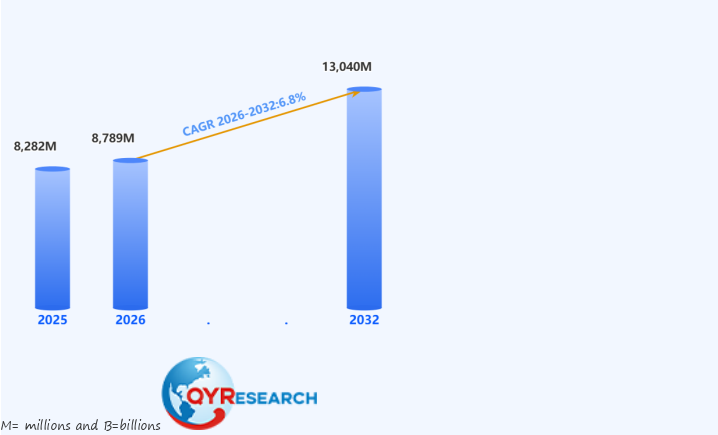
\includegraphics[width=0.8\textwidth]{figures/nfc_market.png}
	\caption{全球 NFC 控制芯片市场规模及预测}
	\label{fig:nfc_market}
\end{figure}

\textbf{2. 技术架构与实现路径}
\begin{itemize}
	\item 通过手机NFC场强感应取电，无需内置电池，确保产品轻薄化（厚度 $<0.8$ 毫米）和免维护。
	\item 签名生成时间控制在50毫秒以内，验证在30毫秒以内，确保总响应时间 $<0.5$ 秒。
	\item 私钥存储于安全芯片受保护存储区，公钥通过安全通道上传至权限管理平台，完成身份绑定。
\end{itemize}

\textbf{3. 商业模式与收入结构} \\
本阶段以\textbf{硬件销售为主导，辅以咨询服务}。NFC贴片参照高安全场景的 DESFire 级产品，毛利率设定在30\%-40\%。同时，为大型企业提供高利润的后量子迁移规划咨询服务。

% 预留图片位置：PQC市场规模图
\begin{figure}[htbp]
	\centering
	% 请将图片命名为 pqc_market.png 并放入 images 文件夹下，然后取消下一行的注释
	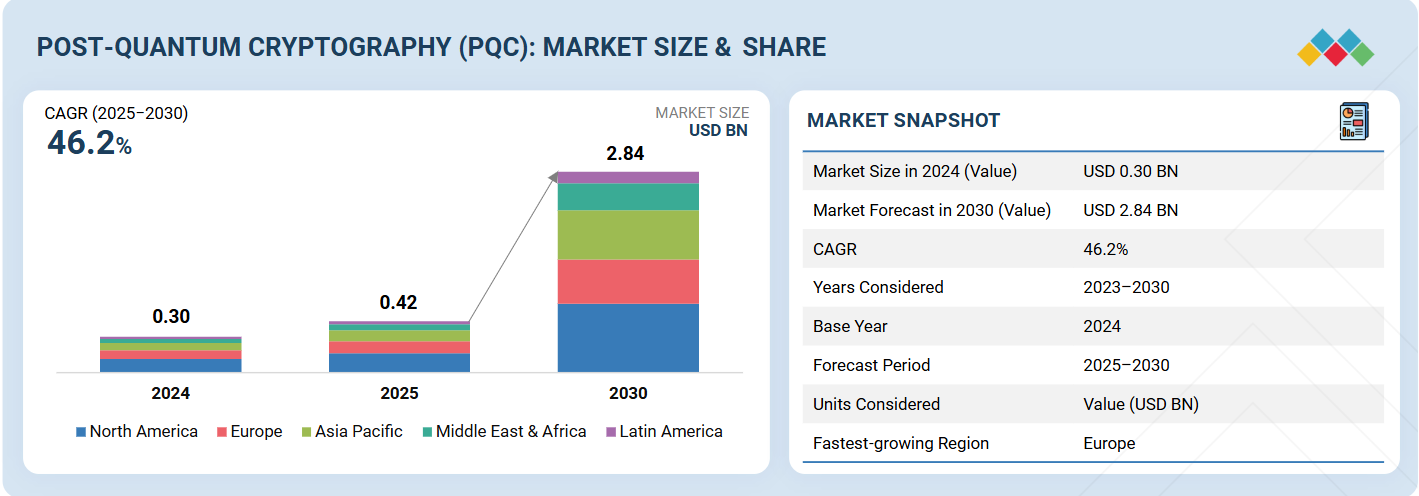
\includegraphics[width=0.85\textwidth]{figures/pqc_market.png}
	\caption{全球后量子密码 (PQC) 市场规模预测}
	\label{fig:pqc_market}
\end{figure}

\subsection{Phase 2：门禁系统升级期（18-36个月）}

\textbf{1. 产品定位与核心价值} \\
核心任务是从单一贴片向\textbf{“贴片+门锁+平台”}一体化系统升级。推出支持PQC算法的终端读卡器/门锁，与PQC贴片配合形成端到端安全链路。根据 Global Growth Insights 数据，基于云的访问控制已占新项目的近33\%。

\textbf{2. 技术架构与实现路径} \\
采用NIST标准：ML-KEM 用于密钥封装，ML-DSA 用于数字签名。系统架构采用\textbf{双栈兼容模式}：同时支持 ML-DSA 和 ECC 签名验证，客户可分批次完成升级，大幅降低迁移门槛。

% 预留图片位置：智能门锁规模图
\begin{figure}[htbp]
	\centering
	% 请将图片命名为 lock_market.png 并放入 images 文件夹下，然后取消下一行的注释
	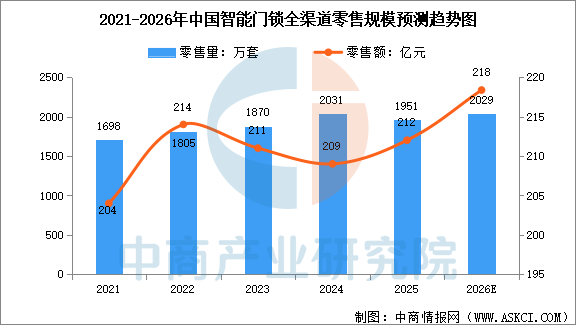
\includegraphics[width=0.8\textwidth]{figures/lock_market.png}
	\caption{2021-2026年中国智能门锁全渠道零售规模预测}
	\label{fig:lock_market}
\end{figure}

\textbf{3. 商业模式与收入结构} \\
从单一硬件向\textbf{“硬件+平台订阅”}转型。平台按节点数收取年费（约 50-80元/年/节点），包含云平台使用费、密钥管理与安全运维。

\subsection{Phase 3：后量子安全平台生态期（36-60个月）}

\textbf{1. 产品定位与核心价值} \\
将安全能力从单一门禁延伸至行业级\textbf{后量子安全中台}。随着NIST标准的确立，PQC生态系统正向云平台、OT设备制造等全领域扩展。

\textbf{2. 平台发布与生态构建} \\
推出“后量子安全服务平台”，提供：密钥全生命周期管理、设备身份认证与权限控制、安全态势感知、安全审计与溯源四大核心模块。

\textbf{3. 商业模式与盈利升级} \\
升级为\textbf{“平台SaaS + 生态分成”}双轮驱动。随着物联网设备的指数级增长，订阅收入规模效应显现。单卡成本将因规模效应及封装工艺优化，进一步降至 5 元以内。

\subsection{三阶段发展路径总结}

\begin{table}[htbp]
	\centering
	\caption{项目三阶段发展路径核心指标总结}
	\label{tab:three_phases_summary}
	\renewcommand{\arraystretch}{1.4}
	\small
	\begin{tabular}{p{1.5cm}p{3.5cm}p{4cm}p{4.5cm}}
		\toprule
		\textbf{维度} & \textbf{Phase 1: 贴片切入期} & \textbf{Phase 2: 系统升级期} & \textbf{Phase 3: 平台生态期} \\
		\midrule
		\textbf{时间} & 0-18个月 & 18-36个月 & 36-60个月 \\
		\textbf{核心产品} & NFC贴片 (ECC/混合) & PQC贴片+终端+云平台 & 行业级后量子安全平台 \\
		\textbf{技术架构} & ECC签名, NFC通信 & ML-KEM + ML-DSA双栈 & 平台化PQC能力, 开放API \\
		\textbf{收入模式} & 硬件销售 + 迁移咨询 & 硬件销售 + \textbf{平台订阅} & \textbf{平台SaaS} + 生态分成 \\
		\textbf{关键指标} & 完成国密认证, 2-3个标杆 & 贴片成本10-15元, ARR达350万 & 单片成本<5元, 净利率>40\% \\
		\textbf{战略目标} & 建立客户基础, 储备需求 & 释放PQC技术价值, 锁定客户 & 构建行业标准, 打造生态 \\
		\bottomrule
	\end{tabular}
\end{table}

\section{财务预测（5年）}

结合PQC市场和门禁市场的增长趋势，编制五年收入预测如下（单位：万元）：

\begin{table}[htbp]
	\centering
	\caption{5年期财务收入结构预测 (万元)}
	\label{tab:financial_forecast_5y}
	\renewcommand{\arraystretch}{1.4}
	\begin{tabular}{cp{2.5cm}cp{3cm}cc}
		\toprule
		\textbf{年度} & \textbf{硬件销售收入} & \textbf{SaaS订阅收入} & \textbf{咨询与服务收入} & \textbf{总收入} & \textbf{同比增速} \\
		\midrule
		\textbf{Y1} & 80 & — & 120 & \textbf{200} & — \\
		\textbf{Y2} & 680 & 8 & 180 & \textbf{868} & \textbf{334\%} \\
		\textbf{Y3} & 2,500 & 80 & 100 & \textbf{2,680} & \textbf{209\%} \\
		\textbf{Y4} & 4,800 & 450 & 50 & \textbf{5,300} & \textbf{98\%} \\
		\textbf{Y5} & 7,500 & 1,200 & 20 & \textbf{8,720} & \textbf{65\%} \\
		\bottomrule
	\end{tabular}
\end{table}

\textbf{关键财务指标分析：}
\begin{enumerate}
	\item \textbf{LTV/CAC 极佳}：以中型企业客户为例，获客成本(CAC)约1.2-1.5万元。按平均订阅周期4年计算，客户生命周期价值(LTV)约7.2万元，\textbf{LTV/CAC比值达 5.0-5.5}，客户单位经济模型极其健康。
	\item \textbf{ARR 快速增长}：经常性收入(ARR)从Y3的80万元增至Y5的1,200万元，三年增长15倍，平台化转型成效显著。
	\item \textbf{盈亏平衡点}：综合盈亏平衡点出现在 \textbf{Y3末至Y4初}。
	\item \textbf{毛利率趋势}：硬件毛利率从25\%提升至56\%，平台SaaS稳定在75\%-80\%，Y5净利润率可达\textbf{40.0\%}。
\end{enumerate}
	% ==========================================
% 第九章
% ==========================================
\chapter{风险分析与应对策略}

后量子密码技术产业化面临多维度不确定性。本章对各类风险进行评估并制定应对策略。不同阶段风险重心存在差异：Phase 1 以市场认知与标准风险为主，Phase 2 以竞争与供应链为主，Phase 3 侧重合规与生态风险。

\section{市场与认知风险}

\textbf{[风险描述]} \\
客户普遍存在“量子攻击尚远，现有方案够用”的认知偏差。此外，对“手机即卡”的NFC贴片安全性存在疑虑。

\textbf{[应对策略]}
\begin{itemize}
	\item \textbf{系统性市场教育}：发布《量子威胁与迁移白皮书》，传递“先捕获后解密”的现实威胁。
	\item \textbf{精准场景切入}：优先突破受国家安全驱动、预算充足的政务、军工、金融刚需场景。
	\item \textbf{开展 TCO 论证}：量化对比物理卡片制卡/补办成本与贴片的长期复用价值，强化经济性。
\end{itemize}

\section{技术与标准风险}

\textbf{[风险描述]} \\
中国PQC国家标准尚未最终确定，存在算法选型合规风险；嵌入式芯片计算资源受限，PQC算法可能影响响应速度。

\textbf{[应对策略]}
\begin{itemize}
	\item \textbf{密码敏捷性架构}：算法模块与业务逻辑解耦，支持固件热更新，无缝切换最终国标算法。
	\item \textbf{双栈兼容模式}：同时支持国密SM系列与PQC算法，任何情况下均保障存量系统的合规准入。
	\item \textbf{硬件加速协处理器}：联合国产芯片厂商开发专用算子加速引擎，确保响应时间 $<0.5$秒。
\end{itemize}

\section{竞争格局风险}

\textbf{[风险描述]} \\
传统安防巨头（如海康、大华）若在PQC技术成熟后快速跟进，可能凭借渠道和品牌优势对项目形成挤压。

\textbf{[应对策略]}
\begin{itemize}
	\item \textbf{建立技术代差与专利壁垒}：当前多数贴片仅支持传统密码，通过 ML-KEM/ML-DSA 构建长期安全护城河。
	\item \textbf{深耕利基市场}：聚焦巨头覆盖不足的高安全物理门禁与工业物联网节点。
	\item \textbf{抢占标准话语权}：深度参与信安标委(TC260)相关工作组及行业白皮书编写，将技术转化为行业标准。
\end{itemize}

\section{客户采纳与需求风险}

\textbf{[风险描述]} \\
大型政企客户采购周期长、决策链条复杂；客户对提前投入防范“未来风险”存在预算顾虑。

\textbf{[应对策略]}
\begin{itemize}
	\item \textbf{增量升级模式}：贴片不替代现有门禁，仅作安全补充；双栈架构支持分批次平滑升级，分担预算压力。
	\item \textbf{绑定合规刚需}：将PQC升级与《等保2.0》、《数据安全法》及关键基础设施保护条例强关联。
	\item \textbf{灯塔工程示范}：打造标杆案例，通过实际交付展示系统可靠性。
\end{itemize}

\section{供应链与成本风险}

\textbf{[风险描述]} \\
单一国产安全芯片供应商可能导致产能和价格波动；PQC算法带来的算力需求可能推高芯片成本。

\textbf{[应对策略]}
\begin{itemize}
	\item \textbf{多供应商策略}：与 2-3 家国产SE芯片厂商建立联合研发与采购机制，分散断供风险。
	\item \textbf{联合定义下一代芯片}：将核心算法固化入芯片底层硬件，在提升性能的同时压缩制造成本。
	\item \textbf{动态安全库存}：建立核心元器件安全库存水位，缓冲短期供应链波动。
\end{itemize}

\section{合规与政策风险}

\textbf{[风险描述]} \\
密码产品受国家严格监管，商密认证、等保要求等动态变化可能影响产品上市节奏。

\textbf{[应对策略]}
\begin{itemize}
	\item \textbf{前置合规评审}：在研发阶段严格对标国密规范，并提前准备EAL4+级认证材料，缩短审查周期。
	\item \textbf{国际国内双合规}：优先服务跨国机构或出口型企业，积累 NIST 与国密体系的双重合规经验。
	\item \textbf{设立专职合规岗}：实时跟踪国家密码管理局政策动态，确保商业模式始终在红线内合法运行。
\end{itemize}
	% ==========================================
% 第四篇 导入过场页
% ==========================================
\cleardoublepage
\thispagestyle{empty}

\vspace*{6cm}

\begin{center}
	{\heiti\erhao 第四篇\quad 我们是谁} 
	\addcontentsline{toc}{part}{第四篇\quad 我们是谁}
	
	\vspace{2cm} 
	
	{\songti\xiaosi \textit{“一支理解密码学底层逻辑、懂得安防行业落地规则、\\ [0.5em] 并在量子安全时代窗口期果断入局的顶尖产学研团队。”}}
\end{center}

\vfill
\cleardoublepage

% ==========================================
% 第十章
% ==========================================
\chapter{团队与融资计划}

本项目的核心壁垒不仅在于前沿的技术架构，更源于我们拥有国内顶尖的密码学产学研落地团队。依托武汉大学国家网络安全学院及计算机学院的深厚学术底蕴，我们构建了一支由国家杰青、重点研发首席科学家领衔，由具备极客精神和商业敏锐度的优秀本科生主导的复合型战队。

\section{核心创始团队}

学生创始团队来自武汉大学密码学与计算机顶尖拔尖班级，兼具底层代码硬实力与商业架构规划能力。

\begin{itemize}
	\item \textbf{张睿恒 | 团队负责人 / 首席执行官 (CEO)} \\
	国家网络安全学院密码试验班 2024级本科生。负责项目的整体战略统筹、底层后量子算法库代码开发与门禁协议适配。曾斩获第十九届“挑战杯”全国大学生课外学术科技作品竞赛\textbf{国家级三等奖}。
	
	\item \textbf{傅承阳 | 核心技术骨干 / 首席技术官 (CTO)} \\
	国家网络安全学院密码试验班 2024级本科生。主导PQC算法的工程化实现与性能极限优化。具备极强的代码落地能力，荣获 \textbf{2025年雷军计算机奖学金}，及2025年“挑战杯”\textbf{国家级三等奖}。
	
	\item \textbf{胡斯舜 | 战略与商业负责人 (COO)} \\
	国家网络安全学院密码科学与技术试验班 2024级本科生。主导项目商业模式设计、财务预测构建及商业计划书撰写，精准把控抗量子基建市场的商业化演进路径。
	
	\item \textbf{汪扬帆 | 商务与路演负责人 (CMO)} \\
	国家网络安全学院密码试验班 2025级本科生。专业绩点稳居\textbf{年级前10\%}，负责对外路演答辩与客户痛点需求挖掘，具备扎实的密码学理论基础与卓越的表达感染力。
	
	\item \textbf{李恺睿 | 运营与合规负责人} \\
	国家网络安全学院密码试验班 2024级本科生。负责项目申报书矩阵构建、知识产权规划与国家密码政策合规性梳理。
	
	\item \textbf{刘芸萱、王一茗 | 品牌视觉与市场宣传总监} \\
	分别来自国家网络安全学院计算机类2025级与新闻与传播学院新闻系2024级（曾获甲等奖学金）。负责公司品牌VI设计、产品UI交互呈现及高质量发布会级路演视觉制作，赋予硬核科技产品卓越的商业美感。
\end{itemize}

\section{顶级科学家顾问委员会}

我们的指导教师团队由国内密码学领域的领军人物组成，为本项目的底层PQC算法、国密合规以及行业标准制定提供了\textbf{无法复制的降维打击能力与学术护城河}。

\begin{description}[labelindent=0pt, leftmargin=1em, style=sameline]
	\item[\textbf{何德彪 教授（首席学术顾问）：}] 武汉大学计算机学院教授、院长，\textbf{国家杰出青年科学基金获得者}。主持国家自然科学基金、科技部重点研发计划等国家级科研项目。近5年，在 IEEE TIFS, IEEE TDSC, ASIACRYPT, PKC 等国际密码学顶级期刊/会议上发表论文40余篇。
	
	\item[\textbf{彭聪 副教授（PQC标准推进顾问）：}] 武汉大学国家网络安全学院副教授，\textbf{国家重点研发计划青年项目首席科学家}。在 ASIACRYPT 等著名期刊发表论文70余篇。其参与实现的“SM2MLKEM768”近期成功获得 \textbf{IANA TLS官方编号：4590}，这是\textbf{我国在后量子密码领域首次获得该项国际认可}，直接赋能本项目底层算法的国际领先性。
	
	\item[\textbf{冯琦 副教授（密码行业标准顾问）：}] 武汉大学国家网络安全学院副教授。发表顶级学术论文40余篇，申请发明专利60余项。\textbf{参与制定/修订密码行业标准2项、成果入选密码行业标准草案}，为项目未来的合规落地与国标主导权奠定坚实基础。
	
	\item[\textbf{李小红 副教授（系统工程顾问）：}] 武汉大学计算机学院软件工程系副教授，曾在美国 Purdue 大学访问。先后主持8个横向课题及多项国家级/国防保密课题，为门禁系统工程化落地与军工级保密需求提供指导。
	
	\item[\textbf{罗敏 教授（网络安全生态顾问）：}] 武汉大学国家网络安全学院副教授、博士生导师。密码科学与技术系党支部书记，CCF区块链专业委员会委员。为项目的物联网生态拓展与分布式安全架构提供前瞻性指引。
\end{description}

\section{融资需求与资金用途}

基于团队现状与规模化扩张需求，我们现正式开启 \textbf{天使轮} 融资。本轮融资将主要用于完成软硬件系统的高度产品化、底层SE安全芯片的联合流片以及首批政企标杆客户的样板工程落地。

\begin{table}[H]
	\centering
	\caption{天使轮融资计划}
	\label{tab:financing_plan}
	\renewcommand{\arraystretch}{1.4}
	\begin{tabular}{p{4cm}p{10cm}}
		\toprule
		\textbf{融资要素} & \textbf{详细说明} \\
		\midrule
		\textbf{融资轮次} & 天使轮 (Angel Round) \\
		\textbf{目标融资金额} & \textbf{1,000万 人民币} \\
		\textbf{出让股权比例} & \textbf{10\% - 15\%} \\
		\textbf{投前估值} & 约 6,000万 - 9,000万 人民币 \\
		\textbf{当前阶段} & 已完成算法底层重构与实验室Demo，初步达成芯片厂商合作意向 \\
		\bottomrule
	\end{tabular}
\end{table}

\begin{table}[H]
	\centering
	\caption{资金用途预算规划}
	\label{tab:fund_usage}
	\renewcommand{\arraystretch}{1.4}
	\begin{tabular}{p{3cm}cp{8.5cm}}
		\toprule
		\textbf{资金用途} & \textbf{占比} & \textbf{具体使用说明} \\
		\midrule
		\textbf{研发与芯片流片} & \textbf{40\%} & 支付流片代工（NRE）及掩膜费用，迭代嵌入式算法底层及硬件协处理器加速模块。 \\
		\textbf{软件平台开发} & \textbf{25\%} & 研发量子安全密钥管理平台（KMS）、敏捷性引擎架构及云端安全态势监控UI/UX。 \\
		\textbf{资质与合规认证} & \textbf{15\%} & 申报并获取国家密码管理局《商用密码产品认证证书》，推进 EAL4+ 安全认证。 \\
		\textbf{市场与标杆工程} & \textbf{10\%} & 在重点军工/政企园区落地2-3个规模化样板工程，开拓全国安防集成商渠道。 \\
		\textbf{日常运营储备} & \textbf{10\%} & 公司日常场地租赁、核心团队薪酬发放及法务/财务合规支出，保障至少18个月现金流。 \\
		\bottomrule
	\end{tabular}
\end{table}



	% ------------------  附录  ------------------
	\newpage
	\phantomsection
	\addcontentsline{toc}{chapter}{附录}
	\section*{附录A\quad 部分核心代码}

\subsection*{A.1 通用多项式乘法（NTT加速）模块}
\textbf{用途}：为ML-KEM和ML-DSA算法提供底层多项式乘法支持，基于NTT（数论变换）实现加速，解决不同算法间代码冗余问题。
\begin{lstlisting}[language=C, caption=通用Poly\_Mul\_NTT模块实现]
#include "ntt.h"
#include "poly.h"

// 模q多项式乘法（NTT加速版）
void Poly_Mul_NTT(poly *r, const poly *a, const poly *b) {
    int i;
    poly t;

    // 对输入多项式执行NTT变换
    ntt(a->coeffs);
    ntt(b->coeffs);

    // 逐元素模乘
    for (i = 0; i < 256; i++) {
        t.coeffs[i] = montgomery_mult(a->coeffs[i], b->coeffs[i]);
    }

    // 逆NTT变换得到结果
    invntt(t.coeffs);
    poly_reduce(&t);
    *r = t;
}

// 多项式归约（防止溢出）
void poly_reduce(poly *a) {
    int i;
    for (i = 0; i < 256; i++) {
        a->coeffs[i] = reduce32(a->coeffs[i]);
    }
}
\end{lstlisting}

\subsection*{A.2 ML-KEM密钥封装/解封装核心接口}
\textbf{用途}：实现后量子密钥封装机制（ML-KEM-768），为PQ-Aliro和PQ-PACE协议提供密钥协商核心功能。
\begin{lstlisting}[language=C, caption=ML-KEM核心接口实现]
#include "ml_kem.h"
#include "randombytes.h"

// 生成ML-KEM密钥对
void ML_KEM_KeyGen(uint8_t *pk, uint8_t *sk) {
    poly sk_poly, pk_poly;
    uint8_t seed[32];
    
    // 生成真随机种子
    randombytes(seed, 32);
    
    // 多项式采样生成私钥
    poly_from_seed(&sk_poly, seed);
    // 生成公钥（pk = H(sk) mod q）
    poly_to_pk(&pk_poly, &sk_poly);
    
    // 序列化密钥
    poly_serialize_sk(sk, &sk_poly);
    poly_serialize_pk(pk, &pk_poly);
}

// 密钥封装（Encaps）
int ML_KEM_Encaps(uint8_t *ct, uint8_t *ss, const uint8_t *pk) {
    poly pk_poly, ct_poly;
    uint8_t seed[32];
    int ret;

    // 解析公钥
    poly_deserialize_pk(&pk_poly, pk);
    // 生成随机种子
    randombytes(seed, 32);
    
    // 生成密文和共享秘密
    ret = poly_encaps(&ct_poly, ss, &pk_poly, seed);
    if (ret != 0) return -1;
    
    // 序列化密文
    poly_serialize_ct(ct, &ct_poly);
    return 0;
}

// 密钥解封装（Decaps）
int ML_KEM_Decaps(uint8_t *ss, const uint8_t *ct, const uint8_t *sk) {
    poly sk_poly, ct_poly;
    
    // 解析私钥和密文
    poly_deserialize_sk(&sk_poly, sk);
    poly_deserialize_ct(&ct_poly, ct);
    
    // 解封装得到共享秘密
    poly_decaps(ss, &ct_poly, &sk_poly);
    return 0;
}
\end{lstlisting}

\subsection*{A.3 ML-DSA签名/验签核心接口}
\textbf{用途}：实现后量子数字签名机制（ML-DSA-44），为PQ-Aliro双向认证、PQ-AA芯片防克隆提供签名验证支持。
\begin{lstlisting}[language=C, caption=ML-DSA核心接口实现]
#include "ml_dsa.h"
#include "shake256.h"

// ML-DSA签名生成
void ML_DSA_Sign(uint8_t *sig, size_t *sig_len, 
                 const uint8_t *msg, size_t msg_len, 
                 const uint8_t *sk) {
    poly sk_poly;
    shake256ctx ctx;
    
    // 解析私钥
    poly_deserialize_sk(&sk_poly, sk);
    
    // 初始化SHAKE256上下文（绑定消息）
    shake256_init(&ctx);
    shake256_absorb(&ctx, msg, msg_len);
    
    // 生成签名
    poly_sign(sig, sig_len, &ctx, &sk_poly);
    
    // 清理上下文
    shake256_free(&ctx);
}

// ML-DSA签名验证
int ML_DSA_Verify(const uint8_t *sig, size_t sig_len, 
                   const uint8_t *msg, size_t msg_len, 
                   const uint8_t *pk) {
    poly pk_poly;
    shake256ctx ctx;
    int ret;
    
    // 解析公钥
    poly_deserialize_pk(&pk_poly, pk);
    
    // 初始化SHAKE256上下文（绑定消息）
    shake256_init(&ctx);
    shake256_absorb(&ctx, msg, msg_len);
    
    // 验证签名
    ret = poly_verify(sig, sig_len, &ctx, &pk_poly);
    
    // 清理上下文
    shake256_free(&ctx);
    return ret; // 0=验证通过，-1=验证失败
}
\end{lstlisting}

\subsection*{A.4 Keccak哈希流式处理接口}
\textbf{用途}：为会话摘要计算、密钥派生提供流式哈希功能，解决嵌入式设备RAM不足导致的大消息处理问题。
\begin{lstlisting}[language=C, caption=Keccak\_State流式接口实现]
#include "keccak.h"

// 初始化Keccak状态
void Keccak_State_Init(keccak_state *state) {
    keccak_init(state, 256); // SHAKE256
}

// 流式更新哈希（增量处理）
void Keccak_State_Update(keccak_state *state, const uint8_t *data, size_t len) {
    keccak_absorb(state, data, len);
}

// 最终化哈希并输出结果
void Keccak_State_Final(keccak_state *state, uint8_t *out, size_t out_len) {
    keccak_squeeze(state, out, out_len);
}

// 计算会话摘要（Transcript Hash）
void calc_transcript_hash(uint8_t *trans_hash, 
                          const uint8_t *auth0_cmd, size_t cmd_len,
                          const uint8_t *auth0_resp, size_t resp_len) {
    keccak_state state;
    
    Keccak_State_Init(&state);
    Keccak_State_Update(&state, auth0_cmd, cmd_len);
    Keccak_State_Update(&state, auth0_resp, resp_len);
    Keccak_State_Final(&state, trans_hash, 32); // 输出32字节摘要
}
\end{lstlisting}


% ==========================================
% 封底 (Back Cover)
% ==========================================
\cleardoublepage % 另起一页
\thispagestyle{empty} % 清除这一页的页眉和页脚，保持纯净

\vspace*{\fill} % 开启顶部弹性空白，实现绝对垂直居中

\begin{center}
	% 前半句使用黑体小2号，彰显气势
	{\heiti\xiaoer 在历史性的密码换代浪潮面前} \\ 
	\vspace{0.8cm}
	{\heiti\xiaoer 技术是最锋利的矛，团队是最坚固的盾。} \\ 
	
	\vspace{2.5cm} % 增加段落呼吸感
	
	% 后半句使用宋体3号，娓娓道来，发出邀请
	{\songti\sanhao 我们已做好全面准备，} \\ 
	\vspace{0.5cm}
	{\songti\sanhao 诚邀顶尖资本共赴这趟重塑未来物理安全边界的伟大征程！}
\end{center}

\vspace*{\fill} % 开启底部弹性空白

	
	
\end{document}